% Options for packages loaded elsewhere
\PassOptionsToPackage{unicode}{hyperref}
\PassOptionsToPackage{hyphens}{url}
\PassOptionsToPackage{dvipsnames,svgnames*,x11names*}{xcolor}
%
\documentclass[
  10pt,
]{article}
\usepackage{lmodern}
\usepackage{amsmath}
\usepackage{ifxetex,ifluatex}
\ifnum 0\ifxetex 1\fi\ifluatex 1\fi=0 % if pdftex
  \usepackage[T1]{fontenc}
  \usepackage[utf8]{inputenc}
  \usepackage{textcomp} % provide euro and other symbols
  \usepackage{amssymb}
\else % if luatex or xetex
  \usepackage{unicode-math}
  \defaultfontfeatures{Scale=MatchLowercase}
  \defaultfontfeatures[\rmfamily]{Ligatures=TeX,Scale=1}
\fi
% Use upquote if available, for straight quotes in verbatim environments
\IfFileExists{upquote.sty}{\usepackage{upquote}}{}
\IfFileExists{microtype.sty}{% use microtype if available
  \usepackage[]{microtype}
  \UseMicrotypeSet[protrusion]{basicmath} % disable protrusion for tt fonts
}{}
\makeatletter
\@ifundefined{KOMAClassName}{% if non-KOMA class
  \IfFileExists{parskip.sty}{%
    \usepackage{parskip}
  }{% else
    \setlength{\parindent}{0pt}
    \setlength{\parskip}{6pt plus 2pt minus 1pt}}
}{% if KOMA class
  \KOMAoptions{parskip=half}}
\makeatother
\usepackage{xcolor}
\IfFileExists{xurl.sty}{\usepackage{xurl}}{} % add URL line breaks if available
\IfFileExists{bookmark.sty}{\usepackage{bookmark}}{\usepackage{hyperref}}
\hypersetup{
  pdftitle={Using R tools for analysis  of primary biodiversity data provided by SBDI},
  pdfauthor={Debora Arlt and Alejandro Ruete  for the Swedish Biodiversity Data Infrastructure},
  colorlinks=true,
  linkcolor=Maroon,
  filecolor=Maroon,
  citecolor=Blue,
  urlcolor=Blue,
  pdfcreator={LaTeX via pandoc}}
\urlstyle{same} % disable monospaced font for URLs
\usepackage[margin=1in]{geometry}
\usepackage{color}
\usepackage{fancyvrb}
\newcommand{\VerbBar}{|}
\newcommand{\VERB}{\Verb[commandchars=\\\{\}]}
\DefineVerbatimEnvironment{Highlighting}{Verbatim}{commandchars=\\\{\}}
% Add ',fontsize=\small' for more characters per line
\usepackage{framed}
\definecolor{shadecolor}{RGB}{248,248,248}
\newenvironment{Shaded}{\begin{snugshade}}{\end{snugshade}}
\newcommand{\AlertTok}[1]{\textcolor[rgb]{0.94,0.16,0.16}{#1}}
\newcommand{\AnnotationTok}[1]{\textcolor[rgb]{0.56,0.35,0.01}{\textbf{\textit{#1}}}}
\newcommand{\AttributeTok}[1]{\textcolor[rgb]{0.77,0.63,0.00}{#1}}
\newcommand{\BaseNTok}[1]{\textcolor[rgb]{0.00,0.00,0.81}{#1}}
\newcommand{\BuiltInTok}[1]{#1}
\newcommand{\CharTok}[1]{\textcolor[rgb]{0.31,0.60,0.02}{#1}}
\newcommand{\CommentTok}[1]{\textcolor[rgb]{0.56,0.35,0.01}{\textit{#1}}}
\newcommand{\CommentVarTok}[1]{\textcolor[rgb]{0.56,0.35,0.01}{\textbf{\textit{#1}}}}
\newcommand{\ConstantTok}[1]{\textcolor[rgb]{0.00,0.00,0.00}{#1}}
\newcommand{\ControlFlowTok}[1]{\textcolor[rgb]{0.13,0.29,0.53}{\textbf{#1}}}
\newcommand{\DataTypeTok}[1]{\textcolor[rgb]{0.13,0.29,0.53}{#1}}
\newcommand{\DecValTok}[1]{\textcolor[rgb]{0.00,0.00,0.81}{#1}}
\newcommand{\DocumentationTok}[1]{\textcolor[rgb]{0.56,0.35,0.01}{\textbf{\textit{#1}}}}
\newcommand{\ErrorTok}[1]{\textcolor[rgb]{0.64,0.00,0.00}{\textbf{#1}}}
\newcommand{\ExtensionTok}[1]{#1}
\newcommand{\FloatTok}[1]{\textcolor[rgb]{0.00,0.00,0.81}{#1}}
\newcommand{\FunctionTok}[1]{\textcolor[rgb]{0.00,0.00,0.00}{#1}}
\newcommand{\ImportTok}[1]{#1}
\newcommand{\InformationTok}[1]{\textcolor[rgb]{0.56,0.35,0.01}{\textbf{\textit{#1}}}}
\newcommand{\KeywordTok}[1]{\textcolor[rgb]{0.13,0.29,0.53}{\textbf{#1}}}
\newcommand{\NormalTok}[1]{#1}
\newcommand{\OperatorTok}[1]{\textcolor[rgb]{0.81,0.36,0.00}{\textbf{#1}}}
\newcommand{\OtherTok}[1]{\textcolor[rgb]{0.56,0.35,0.01}{#1}}
\newcommand{\PreprocessorTok}[1]{\textcolor[rgb]{0.56,0.35,0.01}{\textit{#1}}}
\newcommand{\RegionMarkerTok}[1]{#1}
\newcommand{\SpecialCharTok}[1]{\textcolor[rgb]{0.00,0.00,0.00}{#1}}
\newcommand{\SpecialStringTok}[1]{\textcolor[rgb]{0.31,0.60,0.02}{#1}}
\newcommand{\StringTok}[1]{\textcolor[rgb]{0.31,0.60,0.02}{#1}}
\newcommand{\VariableTok}[1]{\textcolor[rgb]{0.00,0.00,0.00}{#1}}
\newcommand{\VerbatimStringTok}[1]{\textcolor[rgb]{0.31,0.60,0.02}{#1}}
\newcommand{\WarningTok}[1]{\textcolor[rgb]{0.56,0.35,0.01}{\textbf{\textit{#1}}}}
\usepackage{longtable,booktabs}
\usepackage{calc} % for calculating minipage widths
% Correct order of tables after \paragraph or \subparagraph
\usepackage{etoolbox}
\makeatletter
\patchcmd\longtable{\par}{\if@noskipsec\mbox{}\fi\par}{}{}
\makeatother
% Allow footnotes in longtable head/foot
\IfFileExists{footnotehyper.sty}{\usepackage{footnotehyper}}{\usepackage{footnote}}
\makesavenoteenv{longtable}
\usepackage{graphicx}
\makeatletter
\def\maxwidth{\ifdim\Gin@nat@width>\linewidth\linewidth\else\Gin@nat@width\fi}
\def\maxheight{\ifdim\Gin@nat@height>\textheight\textheight\else\Gin@nat@height\fi}
\makeatother
% Scale images if necessary, so that they will not overflow the page
% margins by default, and it is still possible to overwrite the defaults
% using explicit options in \includegraphics[width, height, ...]{}
\setkeys{Gin}{width=\maxwidth,height=\maxheight,keepaspectratio}
% Set default figure placement to htbp
\makeatletter
\def\fps@figure{htbp}
\makeatother
\setlength{\emergencystretch}{3em} % prevent overfull lines
\providecommand{\tightlist}{%
  \setlength{\itemsep}{0pt}\setlength{\parskip}{0pt}}
\setcounter{secnumdepth}{5}
\ifluatex
  \usepackage{selnolig}  % disable illegal ligatures
\fi
\usepackage[]{natbib}
\bibliographystyle{apalike}

\title{Using R tools for analysis of primary biodiversity data provided by SBDI}
\author{Debora Arlt and Alejandro Ruete for the Swedish Biodiversity Data Infrastructure}
\date{2021-05-28}

\begin{document}
\maketitle

{
\hypersetup{linkcolor=}
\setcounter{tocdepth}{2}
\tableofcontents
}
\hypertarget{introduction}{%
\section*{Introduction}\label{introduction}}
\addcontentsline{toc}{section}{Introduction}

Biodiversity resources are increasingly international. The SBDI has made an effort to canalize biodiversity data and resources to help the research community access and analyze Swedish primary biodiversity data. Each research question draws its own challenges which are unique in themselves. Our aim here is to provide a few examples that prompt questions that may be asked at different stages of the process. The validity and appropriateness of a particular method depends on the individual researcher(s). For a comprehensive workflow on how to treat and analyze PBD please refer to our tutorial on \href{https://github.com/biodiversitydata-se/biodiversity-analysis-tools}{biodiversity analysis tool} where we go through the complete workflow Data --\textgreater{} Cleaning --\textgreater{} Fitness evaluation --\textgreater{} Analysis

\hypertarget{r-and-mirroreum}{%
\subsection*{R and Mirroreum}\label{r-and-mirroreum}}
\addcontentsline{toc}{subsection}{R and Mirroreum}

The present tutorial is focused on the statistical programming language R.
R is a free software environment for statistical computing and graphics that is
widely used within the scientific community and where the complete analysis
workflow can be documented in a fully reproducible way.

At SBDI we provide access for researchers and students to \href{https://mirroreum.biodiversitydata.se/}{Mirroreum}
-- an online web-based environment for Reproducible Open Research in the area of
biodiversity analysis. Mirroreum is based on a Free and Open Source stack of software.
Logging in, you immediately get access to a web-based version of R Studio with a
large number of pre-installed packages such as all the packages offered from ROpenSci and more.

Compared to running R Studio on your own machine, Mirroreum offers more
computational resources and a standardized environment where you can rely on all
the relevant packages being installed and the configuration parameters being set
appropriately.
To know more about Mirroreum or to request an account please visit the \href{https://docs.biodiversitydata.se/analyse-data/mirroreum/}{SBDI documentation site}

\hypertarget{sbdi4r---r-package-to-search-an-access-data}{%
\subsection*{SBDI4R - R package to search an access data}\label{sbdi4r---r-package-to-search-an-access-data}}
\addcontentsline{toc}{subsection}{SBDI4R - R package to search an access data}

The SBDI4R package enables the R community to directly access data and resources
hosted by SBDI. The goal is to enable observations of species to be
queried and output in a range of standard formats. It includes some filter functions
that allow you to filter prior to download. It also includes some simple summary
functions, and some function for some simple data exploration. The examples
included in this tutorial also show you how you can continue exploring and analyzing
using other R package.

Please refer to the \href{https://biodiversitydata-se.github.io/SBDI4R}{package documentation}
for details on how to install it. Once installed the SBDI4R package must be loaded
for each new R session:

\begin{Shaded}
\begin{Highlighting}[]
\FunctionTok{library}\NormalTok{(SBDI4R)}
\end{Highlighting}
\end{Shaded}

\hypertarget{customizing-sbdi4r}{%
\subsection*{Customizing SBDI4R}\label{customizing-sbdi4r}}
\addcontentsline{toc}{subsection}{Customizing SBDI4R}

Various aspects of the SBDI4R package can be customized.

\hypertarget{caching}{%
\subsubsection*{Caching}\label{caching}}
\addcontentsline{toc}{subsubsection}{Caching}

SBDI4R can cache most results to local files. This means that if the
same code is run multiple times, the second and subsequent iterations
will be faster. This will also reduce load on the web servers. By
default, this caching is session-based, meaning that the local files are
stored in a temporary directory that is automatically deleted when the R
session is ended. This behaviour can be altered so that caching is
permanent, by setting the caching directory to a non-temporary location.
For example, under Windows, use something like:

\begin{Shaded}
\begin{Highlighting}[]
\FunctionTok{sbdi\_config}\NormalTok{(}\AttributeTok{cache\_directory =} \FunctionTok{file.path}\NormalTok{(}\StringTok{"c:"}\NormalTok{,}\StringTok{"mydata"}\NormalTok{,}\StringTok{"sbdi\_cache"}\NormalTok{)) }\DocumentationTok{\#\# Windows}
\end{Highlighting}
\end{Shaded}

or for Linux:

\begin{Shaded}
\begin{Highlighting}[]
\FunctionTok{sbdi\_config}\NormalTok{(}\AttributeTok{cache\_directory =} \StringTok{"\textasciitilde{}/mydata/sbdi\_cache"}\NormalTok{) }\DocumentationTok{\#\# Linux}
\end{Highlighting}
\end{Shaded}

Note that this directory must exist (you need to create it yourself).

All results will be stored in that cache directory and will be used from
one session to the next. They won't be re-downloaded from the server
unless the user specifically deletes those files or changes the caching
setting to ``refresh''.

If you change the cache\_directory to a permanent location, you may wish
to add something like this to your .Rprofile file, so that it happens
automatically each time the SBDI4R package is loaded:

\begin{Shaded}
\begin{Highlighting}[]
\FunctionTok{setHook}\NormalTok{(}\FunctionTok{packageEvent}\NormalTok{(}\StringTok{"SBDI4R"}\NormalTok{, }\StringTok{"onLoad"}\NormalTok{), }
        \ControlFlowTok{function}\NormalTok{(...) }\FunctionTok{sbdi\_config}\NormalTok{(}\AttributeTok{cache\_directory=}\FunctionTok{file.path}\NormalTok{(}\StringTok{"\textasciitilde{}"}\NormalTok{,}\StringTok{"mydata"}\NormalTok{,}\StringTok{"sbdi\_cache"}\NormalTok{)))}
\end{Highlighting}
\end{Shaded}

Caching can also be turned off entirely by:

\begin{Shaded}
\begin{Highlighting}[]
\FunctionTok{sbdi\_config}\NormalTok{(}\AttributeTok{caching=}\StringTok{"off"}\NormalTok{)}
\end{Highlighting}
\end{Shaded}

or set to ``refresh'', meaning that the cached results will re-downloaded
from the SBDI servers and the cache updated. (This will happen for as
long as caching is set to ``refresh'' --- so you may wish to switch back to
normal ``on'' caching behavior once you have updated your cache with the
data you are working on).

\hypertarget{e-mail-address}{%
\subsubsection*{E-mail address}\label{e-mail-address}}
\addcontentsline{toc}{subsubsection}{E-mail address}

Each download request to SBDI servers is also accompanied by an ``e-mail address''
string that identifies the user making the request. You will need to provide an
email address registered with the SBDI. You can create an account
\href{https://auth.biodiversitydata.se/cas/login}{here}. Once an email is registered
with the SBDI, it should be stored in the config:

\begin{Shaded}
\begin{Highlighting}[]
\FunctionTok{sbdi\_config}\NormalTok{(}\AttributeTok{email=}\StringTok{"your.valid@emailaddress.com"}\NormalTok{)}
\end{Highlighting}
\end{Shaded}

Else you can provide this e-mail address as a parameter directly to
each call of the function occurrences().

\hypertarget{setting-the-download-reason}{%
\subsubsection*{Setting the download reason}\label{setting-the-download-reason}}
\addcontentsline{toc}{subsubsection}{Setting the download reason}

SBDI requires that you provide a reason when downloading occurrence data
(via the SBDI4R \texttt{occurrences()} function). You can provide this as a
parameter directly to each call of \texttt{occurrences()}, or you can set it
once per session using:

\begin{Shaded}
\begin{Highlighting}[]
\FunctionTok{sbdi\_config}\NormalTok{(}\AttributeTok{download\_reason\_id =} \StringTok{"your\_reason\_id"}\NormalTok{)}
\end{Highlighting}
\end{Shaded}

(See \texttt{sbdi\_reasons()} for valid download reasons, e.g.
* 3 for ``education'',
* 7 for ``ecological research'',
* 8 for ``systematic research/taxonomy'',
* 10 for ``testing'')

\emph{NO} other personal identification information is sent. You can see all
configuration settings, including the the user-agent string that is
being used, with the command:

\begin{Shaded}
\begin{Highlighting}[]
\FunctionTok{sbdi\_config}\NormalTok{()}
\end{Highlighting}
\end{Shaded}

\hypertarget{other-options}{%
\subsubsection*{Other options}\label{other-options}}
\addcontentsline{toc}{subsubsection}{Other options}

If you make a request that returns an empty result set (e.g.~an
un-matched name), by default you will simply get an empty data structure
returned to you without any special notification. If you would like to
be warned about empty result sets, you can use:

\begin{Shaded}
\begin{Highlighting}[]
\FunctionTok{sbdi\_config}\NormalTok{(}\AttributeTok{warn\_on\_empty=}\ConstantTok{TRUE}\NormalTok{)}
\end{Highlighting}
\end{Shaded}

\hypertarget{other-packages-needed}{%
\subsection*{Other packages needed}\label{other-packages-needed}}
\addcontentsline{toc}{subsection}{Other packages needed}

Some additional packages are needed for these examples. Install them if necessary
with the following script.

\begin{Shaded}
\begin{Highlighting}[]
\NormalTok{to\_install }\OtherTok{\textless{}{-}} \FunctionTok{c}\NormalTok{(}\StringTok{"BIRDS"}\NormalTok{,}\StringTok{"colorRamps"}\NormalTok{, }\StringTok{"cowplot"}\NormalTok{,}\StringTok{"dplyr"}\NormalTok{,}\StringTok{"ggplot2"}\NormalTok{, }\StringTok{"leaflet"}\NormalTok{,}
                \StringTok{"maps"}\NormalTok{, }\StringTok{"mapdata"}\NormalTok{, }\StringTok{"maptools"}\NormalTok{, }\StringTok{"sf"}\NormalTok{, }\StringTok{"sp"}\NormalTok{, }\StringTok{"rgeos"}\NormalTok{, }\StringTok{"tidyr"}\NormalTok{, }\StringTok{"xts"}\NormalTok{)}
\NormalTok{to\_install }\OtherTok{\textless{}{-}}\NormalTok{ to\_install[}\SpecialCharTok{!}\FunctionTok{sapply}\NormalTok{(to\_install, requireNamespace, }\AttributeTok{quietly=}\ConstantTok{TRUE}\NormalTok{)]}
\ControlFlowTok{if}\NormalTok{(}\FunctionTok{length}\NormalTok{(to\_install)}\SpecialCharTok{\textgreater{}}\DecValTok{0}\NormalTok{)}
    \FunctionTok{install.packages}\NormalTok{(to\_install, }\AttributeTok{repos=}\StringTok{"http://cran.us.r{-}project.org"}\NormalTok{)}
\end{Highlighting}
\end{Shaded}

\hypertarget{your-collaboration-is-appreciated}{%
\subsection*{Your collaboration is appreciated}\label{your-collaboration-is-appreciated}}
\addcontentsline{toc}{subsection}{Your collaboration is appreciated}

Open Source also means that you can contribute. You don't need to know how to program
but every input is appreciated. Did you find something that is not working?
Have suggestions for examples or text? you can always

\begin{enumerate}
\def\labelenumi{\arabic{enumi}.}
\tightlist
\item
  Reach to us via the \href{https://docs.biodiversitydata.se/support/}{support center}
\item
  Submit and issue to the GitHub code repository \href{https://docs.github.com/en/github/managing-your-work-on-github/managing-your-work-with-issues-and-pull-requests/creating-an-issue}{see how}
\item
  Or contribute with your code or documents modifications by \href{https://docs.github.com/en/github/getting-started-with-github/quickstart/fork-a-repo}{``forking''}
  the code and submitting a \href{https://docs.github.com/en/github/collaborating-with-issues-and-pull-requests/proposing-changes-to-your-work-with-pull-requests/creating-a-pull-request-from-a-fork}{``pull request''}
\end{enumerate}

The repositories you can contribute to are:

\begin{itemize}
\tightlist
\item
  Mirroreum \url{https://github.com/mskyttner/mirroreum}\\
\item
  SBDI4R \url{https://github.com/biodiversitydata-se/SBDI4R} (NOTE: we may not develop this package but instead move to a new one)\\
\item
  the general analysis workflows \url{https://github.com/biodiversitydata-se/biodiversity-analysis-tools}\\
\item
  these tutorial \url{https://github.com/biodiversitydata-se/r-tools-tutorial}
\end{itemize}

\hypertarget{example-with-fish-data-from-sers}{%
\section{Example with fish data from SERS}\label{example-with-fish-data-from-sers}}

In this example we are interested in exploring data from a specific data resource -- Swedish Electrofishing Registry - SERS (Institutionen för akvatiska resurser, SLU). This data base has 2.8 M observations starting in the 1950's.

As you may already know, SBDI is a collection of many biodiversity databases. We start by searching for the data resource we are interested in using the function \texttt{pick\_filter()}. This is an interactive query guiding you through the many resources available to filtering your query (data resources, spatial layers, and curated species lists).

\begin{Shaded}
\begin{Highlighting}[]
\FunctionTok{library}\NormalTok{(SBDI4R)}
\NormalTok{fq\_str }\OtherTok{\textless{}{-}} \FunctionTok{pick\_filter}\NormalTok{(}\StringTok{"resource"}\NormalTok{) }
\CommentTok{\# follow the instructions }
\end{Highlighting}
\end{Shaded}

Follow the instruction. Your choices here would have been ``in3'' --\textgreater{} ``dr10''. Your variable \texttt{fq\_str} will now contain a string ``data\_resource\_uid:dr10''.

But we are not interested in the complete database, but on the last 10 years of data. for this we concatenate (add to a vector) another filter string. These will be treated as AND factors.

\begin{Shaded}
\begin{Highlighting}[]
\NormalTok{y1 }\OtherTok{\textless{}{-}} \DecValTok{2008}
\NormalTok{y2 }\OtherTok{\textless{}{-}} \DecValTok{2012}
\NormalTok{fq\_str }\OtherTok{\textless{}{-}} \FunctionTok{c}\NormalTok{(fq\_str, }\FunctionTok{paste0}\NormalTok{(}\StringTok{"year:["}\NormalTok{, y1, }\StringTok{" TO "}\NormalTok{, y2,}\StringTok{"]"}\NormalTok{))}
\CommentTok{\# Note the square brackets are hard limits}
\end{Highlighting}
\end{Shaded}

For references on how to use the filters see SBDI APIS \href{https://api.biodiversitydata.se/?lang=en-US\#ws3}{documentation}.

Using the function \texttt{occurrences()} we can the query for the observations fulfilling our filter. If you haven't specified that in the \texttt{sbdi\_config()} before, you need to pass your email and the download reason.

\begin{Shaded}
\begin{Highlighting}[]
\FunctionTok{library}\NormalTok{(SBDI4R)}
\NormalTok{xf }\OtherTok{\textless{}{-}} \FunctionTok{occurrences}\NormalTok{(}\AttributeTok{fq =}\NormalTok{ fq\_str,}
                 \AttributeTok{email =} \StringTok{"sbdi4r{-}test@biodiversitydata.se"}\NormalTok{, }
                 \AttributeTok{download\_reason\_id =} \DecValTok{10}\NormalTok{)}
\end{Highlighting}
\end{Shaded}

\begin{verbatim}
## Registered S3 methods overwritten by 'ALA4R':
##   method              from  
##   subset.occurrences  SBDI4R
##   summary.occurrences SBDI4R
##   unique.occurrences  SBDI4R
\end{verbatim}

\begin{Shaded}
\begin{Highlighting}[]
\CommentTok{\# Simply summarise all records by data source }
\FunctionTok{table}\NormalTok{(xf}\SpecialCharTok{$}\NormalTok{data}\SpecialCharTok{$}\NormalTok{dataResourceName)}
\end{Highlighting}
\end{Shaded}

\begin{verbatim}
## 
## SLU Aqua  Institute of Freshwater Research Swedish Electrofishing Registry - SERS 
##                                                                             95082
\end{verbatim}

\begin{Shaded}
\begin{Highlighting}[]
\FunctionTok{table}\NormalTok{(xf}\SpecialCharTok{$}\NormalTok{data}\SpecialCharTok{$}\NormalTok{dataResourceID)}
\end{Highlighting}
\end{Shaded}

\begin{verbatim}
## 
##  dr10 
## 95082
\end{verbatim}

\hypertarget{plotting-data-on-a-map}{%
\subsection{Plotting data on a map}\label{plotting-data-on-a-map}}

You can quickly plot all the observations as a PDF file with the function \texttt{ocurrence\_plot()}, one page per species:

\begin{Shaded}
\begin{Highlighting}[]
\FunctionTok{occurrences\_plot}\NormalTok{(xf, }\StringTok{"obsPlot.pdf"}\NormalTok{, }
                 \AttributeTok{grouped=}\ConstantTok{FALSE}\NormalTok{, }
                 \AttributeTok{taxon\_level=}\StringTok{"species"}\NormalTok{, }
                 \AttributeTok{pch=}\StringTok{\textquotesingle{}+\textquotesingle{}}\NormalTok{)}
\end{Highlighting}
\end{Shaded}

Note that the plot is saved to a pdf file in the current working directory. You can find that with \texttt{getwd()}.

\hypertarget{leaflet}{%
\paragraph{Leaflet}\label{leaflet}}

There are many other ways of producing spatial plots in R. The leaflet package provides a simple method of producing browser-based maps with panning, zooming, and background layers:

\begin{Shaded}
\begin{Highlighting}[]
\FunctionTok{library}\NormalTok{(leaflet)}
\CommentTok{\# drop any records with missing lat/lon values}
\NormalTok{xfl }\OtherTok{\textless{}{-}}\NormalTok{ xf}\SpecialCharTok{$}\NormalTok{data[}\SpecialCharTok{!}\FunctionTok{is.na}\NormalTok{(xf}\SpecialCharTok{$}\NormalTok{data}\SpecialCharTok{$}\NormalTok{longitude) }\SpecialCharTok{|} \SpecialCharTok{!}\FunctionTok{is.na}\NormalTok{(xf}\SpecialCharTok{$}\NormalTok{data}\SpecialCharTok{$}\NormalTok{latitude),] }
\NormalTok{marker\_colour }\OtherTok{\textless{}{-}} \FunctionTok{rep}\NormalTok{(}\StringTok{"\#d95f02"}\NormalTok{, }\FunctionTok{nrow}\NormalTok{(xfl))}
\CommentTok{\# blank map, with imagery background}
\FunctionTok{leaflet}\NormalTok{(}\AttributeTok{width =} \StringTok{"100\%"}\NormalTok{) }\SpecialCharTok{\%\textgreater{}\%} 
  \FunctionTok{addProviderTiles}\NormalTok{(}\StringTok{"Esri.WorldImagery"}\NormalTok{) }\SpecialCharTok{\%\textgreater{}\%}
  \CommentTok{\# add markers}
  \FunctionTok{addCircleMarkers}\NormalTok{(xfl}\SpecialCharTok{$}\NormalTok{longitude, xfl}\SpecialCharTok{$}\NormalTok{latitude,  }
                   \AttributeTok{radius =} \DecValTok{1}\NormalTok{, }
                   \AttributeTok{fillOpacity =}\NormalTok{.}\DecValTok{5}\NormalTok{, }
                   \AttributeTok{opacity =} \DecValTok{1}\NormalTok{,}
                   \AttributeTok{col=}\NormalTok{marker\_colour,}
                  \AttributeTok{clusterOptions =} \FunctionTok{markerClusterOptions}\NormalTok{())}
\end{Highlighting}
\end{Shaded}

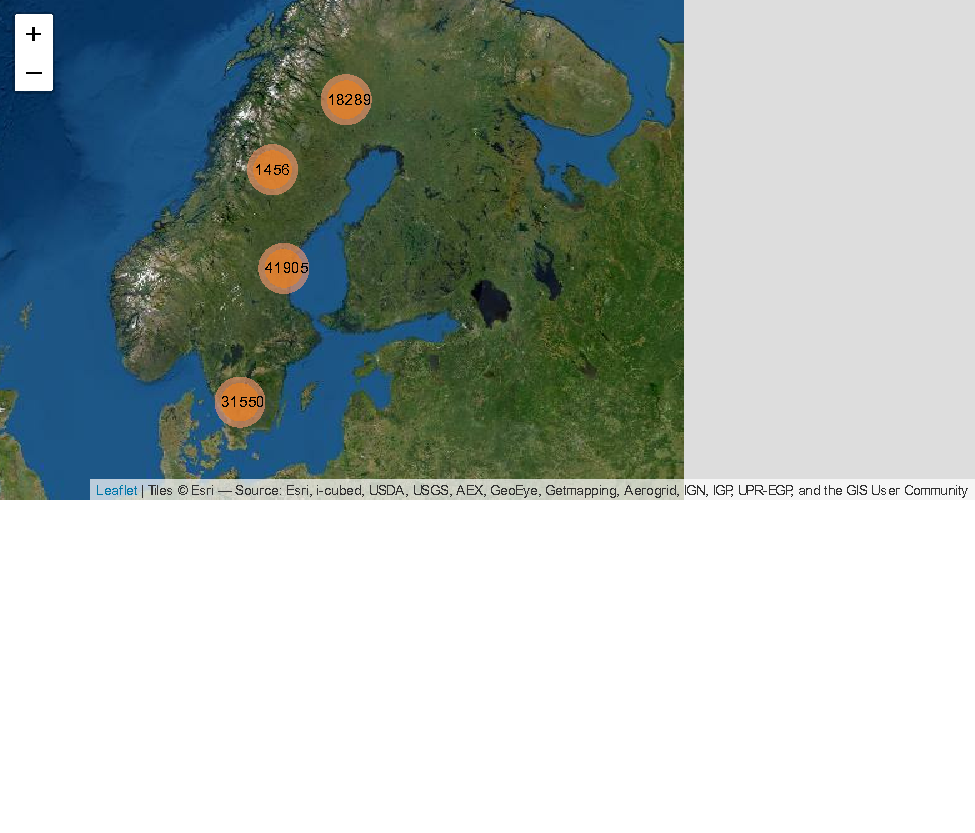
\includegraphics{r-tools-tutorial_files/figure-latex/leaflet-1.pdf}

\hypertarget{temporal-summary}{%
\subsection{Temporal summary}\label{temporal-summary}}

A quick summary over the years reveal a drop in number of records over time.

\begin{Shaded}
\begin{Highlighting}[]
\FunctionTok{table}\NormalTok{(xf}\SpecialCharTok{$}\NormalTok{data}\SpecialCharTok{$}\NormalTok{year)}
\end{Highlighting}
\end{Shaded}

\begin{verbatim}
## 
##  2008  2009  2010  2011  2012 
## 18168 19674 20055 17188 19997
\end{verbatim}

\begin{Shaded}
\begin{Highlighting}[]
\FunctionTok{hist}\NormalTok{(xf}\SpecialCharTok{$}\NormalTok{data}\SpecialCharTok{$}\NormalTok{year, }
     \AttributeTok{breaks =} \FunctionTok{seq}\NormalTok{(y1, y2), }
     \AttributeTok{xlab =} \StringTok{"Year"}\NormalTok{, }
     \AttributeTok{main =} \StringTok{""}\NormalTok{)}
\end{Highlighting}
\end{Shaded}

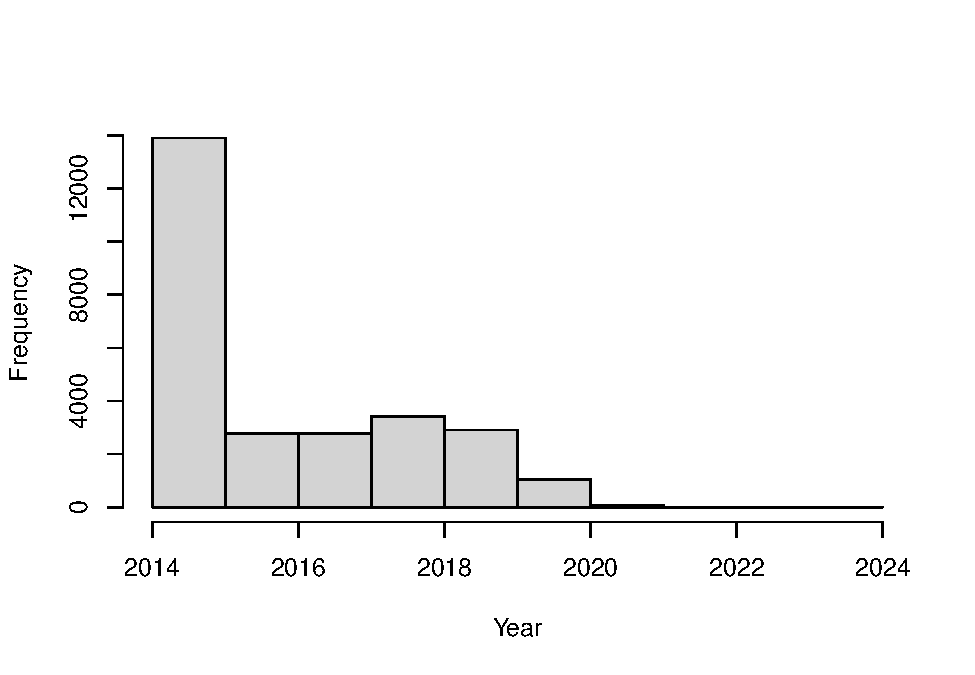
\includegraphics{r-tools-tutorial_files/figure-latex/timeHist-1.pdf}

\hypertarget{species-summary}{%
\subsection{Species summary}\label{species-summary}}

In the same way we can summaries the number of observations for each species, by common or scientific name.

\begin{Shaded}
\begin{Highlighting}[]
\NormalTok{sppTab }\OtherTok{\textless{}{-}} \FunctionTok{table}\NormalTok{(xf}\SpecialCharTok{$}\NormalTok{data}\SpecialCharTok{$}\NormalTok{commonName)}
\NormalTok{sppDF }\OtherTok{\textless{}{-}} \FunctionTok{as.data.frame}\NormalTok{(sppTab)}
\FunctionTok{colnames}\NormalTok{(sppDF)[}\DecValTok{1}\NormalTok{] }\OtherTok{\textless{}{-}} \StringTok{"species"}
\FunctionTok{head}\NormalTok{(sppDF)}
\end{Highlighting}
\end{Shaded}

\begin{verbatim}
##           species Freq
## 1                   66
## 2 Alpine bullhead 4615
## 3 American burbot 7081
## 4        Aral asp    6
## 5     Arctic char   46
## 6    aurora trout  856
\end{verbatim}

\begin{Shaded}
\begin{Highlighting}[]
\NormalTok{sppTab }\OtherTok{\textless{}{-}} \FunctionTok{table}\NormalTok{(xf}\SpecialCharTok{$}\NormalTok{data}\SpecialCharTok{$}\NormalTok{scientificName)}
\NormalTok{sppDF }\OtherTok{\textless{}{-}} \FunctionTok{as.data.frame}\NormalTok{(sppTab)}
\FunctionTok{colnames}\NormalTok{(sppDF)[}\DecValTok{1}\NormalTok{] }\OtherTok{\textless{}{-}} \StringTok{"species"}
\FunctionTok{head}\NormalTok{(sppDF)}
\end{Highlighting}
\end{Shaded}

\begin{verbatim}
##                                species Freq
## 1       Abramis brama (Linnaeus, 1758)   61
## 2   Alburnus alburnus (Linnaeus, 1758)  660
## 3   Anguilla anguilla (Linnaeus, 1758) 2140
## 4                            Astacidae  100
## 5     Astacus astacus (Linnaeus, 1758)  618
## 6 Barbatula barbatula (Linnaeus, 1758)  620
\end{verbatim}

Perhaps, you need to send this table as a .CSV file to a colleague.

\begin{Shaded}
\begin{Highlighting}[]
\FunctionTok{write.csv}\NormalTok{(sppDF, }\StringTok{"SERS\_species\_summary.csv"}\NormalTok{)}
\CommentTok{\# }\AlertTok{NOTE}\CommentTok{: again this will be saved on your working directory}
\end{Highlighting}
\end{Shaded}

\hypertarget{spatial-biodiversity-analysis}{%
\subsection{Spatial biodiversity analysis}\label{spatial-biodiversity-analysis}}

Let's now ask: how does the species richness vary across Sweden? In this case we want to summarise occurrences species-wise over a defined grid instead of plotting every observation point. First we need to overlay the observations with a grid. In this case, the standard Swedish grids at 50, 25, 10 and 5 km are provided as data in the SBDI4R package (with Coordinate Reference System = WGS84, EPSG:4326).

\begin{Shaded}
\begin{Highlighting}[]
\FunctionTok{library}\NormalTok{(sp) }\CommentTok{\# the function coordinates() and proj4string() are in sp}
\end{Highlighting}
\end{Shaded}

\begin{verbatim}
## Warning: package 'sp' was built under R version 4.0.3
\end{verbatim}

\begin{Shaded}
\begin{Highlighting}[]
\FunctionTok{library}\NormalTok{(rgeos) }\CommentTok{\# the function over() is in package rgeos}
\end{Highlighting}
\end{Shaded}

\begin{verbatim}
## rgeos version: 0.5-5, (SVN revision 640)
##  GEOS runtime version: 3.8.0-CAPI-1.13.1 
##  Linking to sp version: 1.4-2 
##  Polygon checking: TRUE
\end{verbatim}

\begin{Shaded}
\begin{Highlighting}[]
\CommentTok{\# load some shapes over Sweden\textquotesingle{}s political borders}
\FunctionTok{data}\NormalTok{(}\StringTok{"swe\_wgs84"}\NormalTok{, }\AttributeTok{package=}\StringTok{"SBDI4R"}\NormalTok{, }\AttributeTok{envir=}\FunctionTok{environment}\NormalTok{())}
\CommentTok{\# A standard 50km grid}
\FunctionTok{data}\NormalTok{(}\StringTok{"Sweden\_Grid\_50km\_Wgs84"}\NormalTok{, }\AttributeTok{package=}\StringTok{"SBDI4R"}\NormalTok{, }\AttributeTok{envir=}\FunctionTok{environment}\NormalTok{())}

\NormalTok{grid }\OtherTok{\textless{}{-}}\NormalTok{ Sweden\_Grid\_50km\_Wgs84}

\CommentTok{\# make the observations spatial}
\CommentTok{\# }\AlertTok{NOTE}\CommentTok{: make sure there are no NAs on either column defining the coordinates}
\CommentTok{\# xf$data[!is.na(xf$data$longitude) | !is.na(xf$data$latitude),]}

\NormalTok{obs }\OtherTok{\textless{}{-}} \FunctionTok{as.data.frame}\NormalTok{(xf}\SpecialCharTok{$}\NormalTok{data)}
\FunctionTok{coordinates}\NormalTok{(obs) }\OtherTok{\textless{}{-}}\NormalTok{ obs[,}\FunctionTok{c}\NormalTok{(}\StringTok{"longitude"}\NormalTok{,}\StringTok{"latitude"}\NormalTok{)]}
\NormalTok{wkt }\OtherTok{\textless{}{-}}\NormalTok{ sf}\SpecialCharTok{::}\FunctionTok{st\_crs}\NormalTok{(}\DecValTok{4326}\NormalTok{)[[}\DecValTok{2}\NormalTok{]]}
\FunctionTok{proj4string}\NormalTok{(obs) }\OtherTok{\textless{}{-}}\NormalTok{ sp}\SpecialCharTok{::}\FunctionTok{CRS}\NormalTok{(wkt) }\CommentTok{\#CRS("+init=epsg:4326")}

\NormalTok{nObs }\OtherTok{\textless{}{-}} \FunctionTok{nrow}\NormalTok{(obs)}

\CommentTok{\# overlay the data with the grid}
\NormalTok{ObsInGridList }\OtherTok{\textless{}{-}} \FunctionTok{over}\NormalTok{(grid, obs, }\AttributeTok{returnList=}\ConstantTok{TRUE}\NormalTok{)}
\NormalTok{wNonEmpty }\OtherTok{\textless{}{-}} \FunctionTok{unname}\NormalTok{( }\FunctionTok{which}\NormalTok{( }\FunctionTok{unlist}\NormalTok{(}\FunctionTok{lapply}\NormalTok{(ObsInGridList, nrow)) }\SpecialCharTok{!=} \DecValTok{0}\NormalTok{) )}
\ControlFlowTok{if}\NormalTok{(}\FunctionTok{length}\NormalTok{(wNonEmpty)}\SpecialCharTok{==}\DecValTok{0}\NormalTok{) }\FunctionTok{message}\NormalTok{(}\StringTok{"Observations don\textquotesingle{}t overlap any grid cell."}\NormalTok{)}
\end{Highlighting}
\end{Shaded}

The result \texttt{ObsInGridList} is a \texttt{list} object with a subset of the data on each grid. Now summarise occurrences within grid cells:

\begin{Shaded}
\begin{Highlighting}[]
\CommentTok{\# check n the total number of observations}
\FunctionTok{sum}\NormalTok{(}\FunctionTok{unlist}\NormalTok{(}\FunctionTok{lapply}\NormalTok{(ObsInGridList, nrow)))}
\end{Highlighting}
\end{Shaded}

\begin{verbatim}
## [1] 95082
\end{verbatim}

\begin{Shaded}
\begin{Highlighting}[]
\CommentTok{\# apply a summary over the grid cells }
\NormalTok{nCells }\OtherTok{\textless{}{-}} \FunctionTok{length}\NormalTok{(ObsInGridList)}

\NormalTok{res }\OtherTok{\textless{}{-}} \FunctionTok{data.frame}\NormalTok{(}\StringTok{"nObs"}\OtherTok{=}\FunctionTok{as.numeric}\NormalTok{(}\FunctionTok{rep}\NormalTok{(}\ConstantTok{NA}\NormalTok{,nCells)),}
                  \StringTok{"nYears"}\OtherTok{=}\FunctionTok{as.numeric}\NormalTok{(}\FunctionTok{rep}\NormalTok{(}\ConstantTok{NA}\NormalTok{,nCells)),}
                  \StringTok{"nSpp"}\OtherTok{=}\FunctionTok{as.numeric}\NormalTok{(}\FunctionTok{rep}\NormalTok{(}\ConstantTok{NA}\NormalTok{,nCells)),}
                  \AttributeTok{row.names =} \FunctionTok{row.names}\NormalTok{(grid),}
                  \AttributeTok{stringsAsFactors =} \ConstantTok{FALSE}\NormalTok{)}

\NormalTok{cols2use }\OtherTok{\textless{}{-}} \FunctionTok{c}\NormalTok{(}\StringTok{"scientificName"}\NormalTok{, }\StringTok{"year"}\NormalTok{)}

\NormalTok{dataRes }\OtherTok{\textless{}{-}} \FunctionTok{lapply}\NormalTok{(ObsInGridList[wNonEmpty], }
                  \ControlFlowTok{function}\NormalTok{(x)\{}
\NormalTok{                    x }\OtherTok{\textless{}{-}}\NormalTok{ x[,cols2use]}
                    \FunctionTok{colnames}\NormalTok{(x) }\OtherTok{\textless{}{-}} \FunctionTok{c}\NormalTok{(}\StringTok{"scientificName"}\NormalTok{, }\StringTok{"year"}\NormalTok{)}
                    \FunctionTok{return}\NormalTok{(}\FunctionTok{c}\NormalTok{(}\StringTok{"nObs"} \OtherTok{=} \FunctionTok{length}\NormalTok{(x[,}\StringTok{"scientificName"}\NormalTok{]),}
                             \StringTok{"nYears"} \OtherTok{=} \FunctionTok{length}\NormalTok{(}\FunctionTok{unique}\NormalTok{(x[,}\StringTok{"year"}\NormalTok{])),}
                             \StringTok{"nSpp"} \OtherTok{=} \FunctionTok{length}\NormalTok{(}\FunctionTok{unique}\NormalTok{(x[,}\StringTok{"scientificName"}\NormalTok{]))}
\NormalTok{                             )}
\NormalTok{                           )}
\NormalTok{                    \}}
\NormalTok{                  )}

\NormalTok{dataRes }\OtherTok{\textless{}{-}} \FunctionTok{as.data.frame}\NormalTok{(dplyr}\SpecialCharTok{::}\FunctionTok{bind\_rows}\NormalTok{(dataRes, }\AttributeTok{.id =} \StringTok{"gridID"}\NormalTok{))}

\NormalTok{res[wNonEmpty,] }\OtherTok{\textless{}{-}}\NormalTok{ dataRes[,}\SpecialCharTok{{-}}\DecValTok{1}\NormalTok{]}

\NormalTok{resSp }\OtherTok{\textless{}{-}}\NormalTok{ sp}\SpecialCharTok{::}\FunctionTok{SpatialPolygonsDataFrame}\NormalTok{(grid, res)}
\end{Highlighting}
\end{Shaded}

And finally plot the grid summary as a map:

\begin{Shaded}
\begin{Highlighting}[]
\NormalTok{palBW }\OtherTok{\textless{}{-}}\NormalTok{ leaflet}\SpecialCharTok{::}\FunctionTok{colorNumeric}\NormalTok{(}\FunctionTok{c}\NormalTok{(}\StringTok{"white"}\NormalTok{, }\StringTok{"navyblue"}\NormalTok{),}
                               \FunctionTok{c}\NormalTok{(}\DecValTok{0}\NormalTok{, }\FunctionTok{max}\NormalTok{(resSp}\SpecialCharTok{@}\NormalTok{data}\SpecialCharTok{$}\NormalTok{nSpp, }\AttributeTok{na.rm =} \ConstantTok{TRUE}\NormalTok{)),}
                               \AttributeTok{na.color =} \StringTok{"transparent"}\NormalTok{)}
\NormalTok{oldpar }\OtherTok{\textless{}{-}} \FunctionTok{par}\NormalTok{()}
\FunctionTok{par}\NormalTok{(}\AttributeTok{mar =} \FunctionTok{c}\NormalTok{(}\DecValTok{1}\NormalTok{,}\DecValTok{1}\NormalTok{,}\DecValTok{0}\NormalTok{,}\DecValTok{0}\NormalTok{))}
\FunctionTok{plot}\NormalTok{(resSp, }\AttributeTok{col=}\FunctionTok{palBW}\NormalTok{(resSp}\SpecialCharTok{@}\NormalTok{data}\SpecialCharTok{$}\NormalTok{nSpp), }\AttributeTok{border =} \ConstantTok{NA}\NormalTok{)}
\FunctionTok{plot}\NormalTok{(swe\_wgs84}\SpecialCharTok{$}\NormalTok{Border, }\AttributeTok{border=}\DecValTok{1}\NormalTok{, }\AttributeTok{lwd=}\DecValTok{1}\NormalTok{, }\AttributeTok{add=}\NormalTok{T)}
\FunctionTok{legend}\NormalTok{(}\StringTok{"bottomleft"}\NormalTok{, }
       \AttributeTok{legend =} \FunctionTok{round}\NormalTok{(}\FunctionTok{seq}\NormalTok{(}\DecValTok{0}\NormalTok{, }\FunctionTok{max}\NormalTok{(resSp}\SpecialCharTok{@}\NormalTok{data}\SpecialCharTok{$}\NormalTok{nSpp, }\AttributeTok{na.rm =} \ConstantTok{TRUE}\NormalTok{), }\AttributeTok{length.out =} \DecValTok{5}\NormalTok{)),}
       \AttributeTok{col =} \FunctionTok{palBW}\NormalTok{(}\FunctionTok{seq}\NormalTok{(}\DecValTok{0}\NormalTok{, }\FunctionTok{max}\NormalTok{(resSp}\SpecialCharTok{@}\NormalTok{data}\SpecialCharTok{$}\NormalTok{nSpp, }\AttributeTok{na.rm =} \ConstantTok{TRUE}\NormalTok{), }\AttributeTok{length.out =} \DecValTok{5}\NormalTok{)),}
       \AttributeTok{title =} \StringTok{"Number of }\SpecialCharTok{\textbackslash{}n}\StringTok{species"}\NormalTok{, }\AttributeTok{pch =} \DecValTok{15}\NormalTok{, }\AttributeTok{bty=}\StringTok{"n"}\NormalTok{)}
\end{Highlighting}
\end{Shaded}

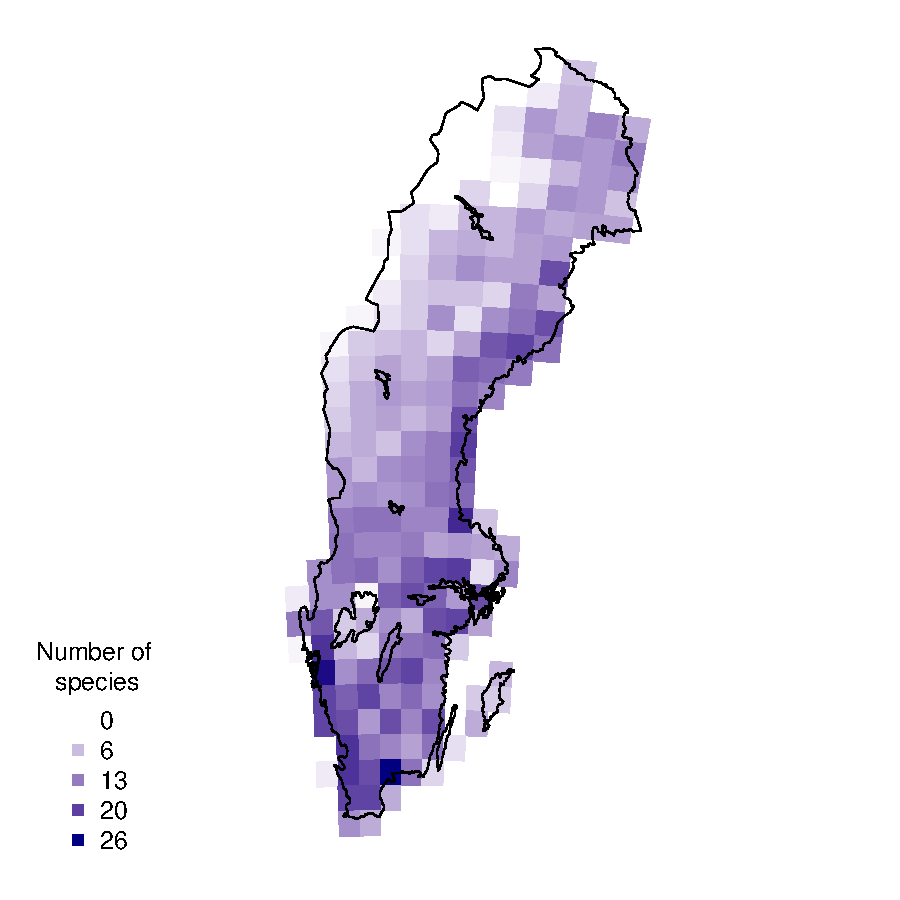
\includegraphics{r-tools-tutorial_files/figure-latex/grid-1.pdf}

\begin{Shaded}
\begin{Highlighting}[]
\FunctionTok{suppressWarnings}\NormalTok{(}\FunctionTok{par}\NormalTok{(oldpar))}
\end{Highlighting}
\end{Shaded}

We can go further by gathering the observations by latitude.

\begin{Shaded}
\begin{Highlighting}[]
\FunctionTok{library}\NormalTok{(dplyr)}
\FunctionTok{library}\NormalTok{(tidyr)}
\NormalTok{xgridded }\OtherTok{\textless{}{-}}\NormalTok{ xf}\SpecialCharTok{$}\NormalTok{data }\SpecialCharTok{\%\textgreater{}\%}
    \DocumentationTok{\#\# discard genus{-} and higher{-}level records}
    \FunctionTok{filter}\NormalTok{(rank }\SpecialCharTok{\%in\%} \FunctionTok{c}\NormalTok{(}\StringTok{"species"}\NormalTok{, }\StringTok{"subspecies"}\NormalTok{, }\StringTok{"variety"}\NormalTok{, }\StringTok{"form"}\NormalTok{, }\StringTok{"cultivar"}\NormalTok{)) }\SpecialCharTok{\%\textgreater{}\%}
    \FunctionTok{mutate}\NormalTok{(}\AttributeTok{longitude =} \FunctionTok{round}\NormalTok{(longitude }\SpecialCharTok{*} \DecValTok{4}\NormalTok{)}\SpecialCharTok{/}\DecValTok{4}\NormalTok{, }
           \AttributeTok{latitude =} \FunctionTok{round}\NormalTok{(latitude }\SpecialCharTok{*} \DecValTok{4}\NormalTok{)}\SpecialCharTok{/}\DecValTok{4}\NormalTok{) }\SpecialCharTok{\%\textgreater{}\%}
    \FunctionTok{group\_by}\NormalTok{(longitude,latitude) }\SpecialCharTok{\%\textgreater{}\%}
    \DocumentationTok{\#\# subset to vars of interest}
    \FunctionTok{select}\NormalTok{(longitude, latitude, species) }\SpecialCharTok{\%\textgreater{}\%}
    \DocumentationTok{\#\# take one row per cell per species (presence)}
    \FunctionTok{distinct}\NormalTok{() }\SpecialCharTok{\%\textgreater{}\%}
    \DocumentationTok{\#\# calculate species richness}
    \FunctionTok{mutate}\NormalTok{(}\AttributeTok{richness=}\FunctionTok{n}\NormalTok{()) }\SpecialCharTok{\%\textgreater{}\%}
    \DocumentationTok{\#\# convert to wide format (sites by species)}
    \FunctionTok{mutate}\NormalTok{(}\AttributeTok{present=}\DecValTok{1}\NormalTok{) }\SpecialCharTok{\%\textgreater{}\%}
    \FunctionTok{do}\NormalTok{(tidyr}\SpecialCharTok{::}\FunctionTok{pivot\_wider}\NormalTok{(}\AttributeTok{data=}\NormalTok{.,  }\AttributeTok{names\_from=}\NormalTok{species, }\AttributeTok{values\_from=}\NormalTok{present, }\AttributeTok{values\_fill=}\DecValTok{0}\NormalTok{)) }\SpecialCharTok{\%\textgreater{}\%}
    \FunctionTok{ungroup}\NormalTok{()}
\DocumentationTok{\#\# where a species was not present, it will have NA: convert these to 0}
\NormalTok{sppcols }\OtherTok{\textless{}{-}} \FunctionTok{setdiff}\NormalTok{(}\FunctionTok{names}\NormalTok{(xgridded),}
                   \FunctionTok{c}\NormalTok{(}\StringTok{"longitude"}\NormalTok{, }\StringTok{"latitude"}\NormalTok{, }\StringTok{"richness"}\NormalTok{))}
\NormalTok{xgridded }\OtherTok{\textless{}{-}}\NormalTok{ xgridded }\SpecialCharTok{\%\textgreater{}\%} 
  \FunctionTok{mutate\_at}\NormalTok{(sppcols, }\ControlFlowTok{function}\NormalTok{(z) }\FunctionTok{ifelse}\NormalTok{(}\FunctionTok{is.na}\NormalTok{(z), }\DecValTok{0}\NormalTok{, z))}
\end{Highlighting}
\end{Shaded}

And plot it accordingly

\begin{Shaded}
\begin{Highlighting}[]
\FunctionTok{library}\NormalTok{(ggplot2)}

\FunctionTok{ggplot}\NormalTok{(xgridded, }\FunctionTok{aes}\NormalTok{(latitude, richness)) }\SpecialCharTok{+} 
  \FunctionTok{labs}\NormalTok{(}\AttributeTok{x =} \StringTok{"Latitude (º)"}\NormalTok{, }
       \AttributeTok{y =} \StringTok{"Species richness"}\NormalTok{) }\SpecialCharTok{+}
  \FunctionTok{lims}\NormalTok{(}\AttributeTok{y =} \FunctionTok{c}\NormalTok{(}\DecValTok{0}\NormalTok{,}\DecValTok{20}\NormalTok{)) }\SpecialCharTok{+}
  \FunctionTok{geom\_point}\NormalTok{() }\SpecialCharTok{+} 
  \FunctionTok{theme\_bw}\NormalTok{()}
\end{Highlighting}
\end{Shaded}

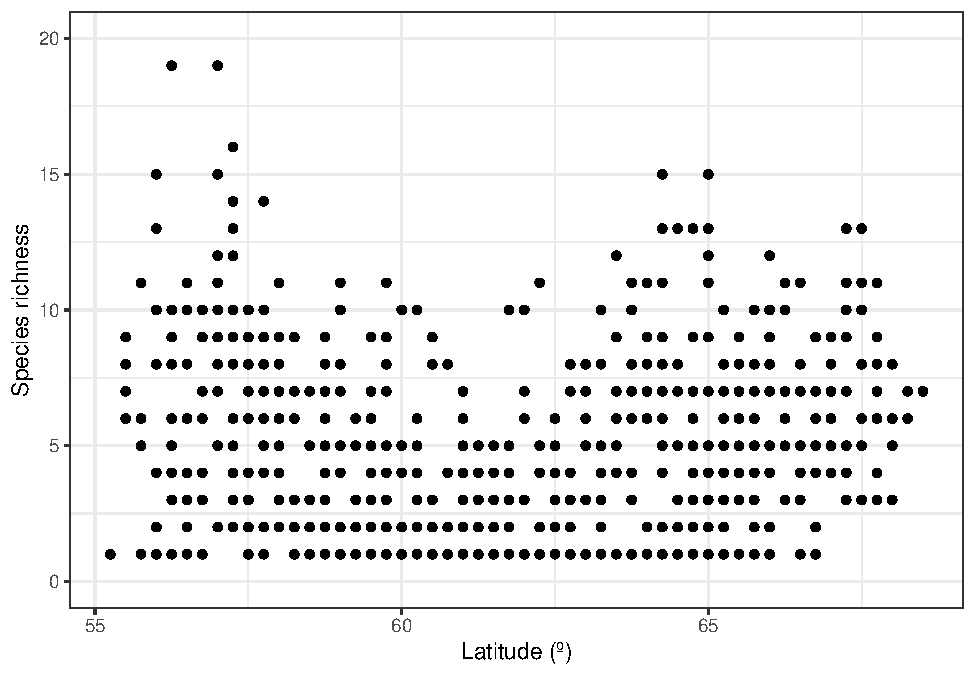
\includegraphics{r-tools-tutorial_files/figure-latex/plot_richLat-1.pdf}

\hypertarget{example-with-opportunistic-data-on-dragonflies}{%
\section{Example with opportunistic data on Dragonflies}\label{example-with-opportunistic-data-on-dragonflies}}

In this example we are interested in exploring opportunistically collected data
from the Swedish citizen science observation data portal - Artportalen.

\hypertarget{name-searching}{%
\subsection{Name searching}\label{name-searching}}

To begin, we want be sure there is an unequivocal way to find the species within
the order Odonata and nothing else, so let's search for it:

\begin{Shaded}
\begin{Highlighting}[]
\FunctionTok{library}\NormalTok{(SBDI4R)}
\NormalTok{sx }\OtherTok{\textless{}{-}} \FunctionTok{search\_fulltext}\NormalTok{(}\StringTok{"odonata"}\NormalTok{)}
\end{Highlighting}
\end{Shaded}

\begin{verbatim}
## [1] "https://species.biodiversitydata.se/ws/search.json?q=odonata&fq=idxtype%3ATAXON"
\end{verbatim}

\begin{Shaded}
\begin{Highlighting}[]
\NormalTok{sx}
\end{Highlighting}
\end{Shaded}

\begin{verbatim}
## Search metadata:
##   totalRecords queryTitle
## 1            5    odonata
## 
## Facet results:
## [1] "NULL"
## 
## Search results:
##   name                                      commonNameSingle rank     
## 1 "Odonata associated gemycircularvirus 1"  ""               "species"
## 2 "Odonata associated gemycircularvirus 2"  ""               "species"
## 3 "Bdellodes odonata Wallace & Mahon, 1976" ""               "species"
## 4 "Odonata"                                 ""               "order"  
## 5 "Ramalina fastigiata var. odonata Hue"    ""               "variety"
##   guid      
## 1 "9829523" 
## 2 "10072832"
## 3 "8062407" 
## 4 "789"     
## 5 "7367071"
\end{verbatim}

we see there that other taxonomic definitions appear too, but only one order.
Let's refine the search. To know the names of the search fields (that may not be
the same as returned column names) we can use the function \texttt{sbdi\_fields(fields\_type\ =\ "general")}.
The search field we are looking for is ``order\_s''.

\begin{Shaded}
\begin{Highlighting}[]
\NormalTok{sx }\OtherTok{\textless{}{-}} \FunctionTok{search\_fulltext}\NormalTok{(}\AttributeTok{fq=}\StringTok{"order\_s:Odonata"}\NormalTok{, }\AttributeTok{page\_size =} \DecValTok{10}\NormalTok{)}
\end{Highlighting}
\end{Shaded}

\begin{verbatim}
## [1] "https://species.biodiversitydata.se/ws/search.json?fq=order_s%3AOdonata&fq=idxtype%3ATAXON&pageSize=10"
\end{verbatim}

\begin{Shaded}
\begin{Highlighting}[]
\NormalTok{sx}\SpecialCharTok{$}\NormalTok{data[,}\FunctionTok{c}\NormalTok{( }\StringTok{"name"}\NormalTok{,}\StringTok{"scientificName"}\NormalTok{, }\StringTok{"guid"}\NormalTok{, }\StringTok{"rank"}\NormalTok{)]}
\end{Highlighting}
\end{Shaded}

\begin{verbatim}
##                                          name
## 1                 Gomphomacromia Brauer, 1864
## 2                Austropetalia Tillyard, 1916
## 3                  Sogjutella Pritykina, 1980
## 4                     Neuragrion Karsch, 1891
## 5               Xamenophlebia Pritykina, 1981
## 6                Lauromacromia Geijskes, 1970
## 7                      Sympetrum Newman, 1833
## 8  Corduliochlora Marinov & Seidenbusch, 2007
## 9              Torrenticnemis Lieftinck, 1949
## 10                  Cyanallagma Kennedy, 1920
##                                scientificName    guid  rank
## 1                 Gomphomacromia Brauer, 1864 1429753 genus
## 2                Austropetalia Tillyard, 1916 1426725 genus
## 3                  Sogjutella Pritykina, 1980 4799335 genus
## 4                     Neuragrion Karsch, 1891 4302686 genus
## 5               Xamenophlebia Pritykina, 1981 4799353 genus
## 6                Lauromacromia Geijskes, 1970 1429769 genus
## 7                      Sympetrum Newman, 1833 1428195 genus
## 8  Corduliochlora Marinov & Seidenbusch, 2007 4798599 genus
## 9              Torrenticnemis Lieftinck, 1949 1423625 genus
## 10                  Cyanallagma Kennedy, 1920 1423468 genus
\end{verbatim}

Now we can download the taxonomic data (note that the search is case-sensitive):

\begin{Shaded}
\begin{Highlighting}[]
\NormalTok{tx }\OtherTok{\textless{}{-}} \FunctionTok{taxinfo\_download}\NormalTok{(}\StringTok{"order\_s:Odonata"}\NormalTok{, }
                       \AttributeTok{fields =} \FunctionTok{c}\NormalTok{(}\StringTok{"guid"}\NormalTok{, }\StringTok{"order\_s"}\NormalTok{,}\StringTok{"genus\_s"}\NormalTok{, }\StringTok{"specificEpithet\_s"}\NormalTok{, }
                                  \StringTok{"scientificName"}\NormalTok{,  }\StringTok{"canonicalName\_s"}\NormalTok{, }\StringTok{"rank"}\NormalTok{), }
                       \AttributeTok{verbose =} \ConstantTok{FALSE}\NormalTok{)}
\NormalTok{tx }\OtherTok{\textless{}{-}}\NormalTok{ tx[tx}\SpecialCharTok{$}\NormalTok{rank }\SpecialCharTok{==} \StringTok{"species"} \SpecialCharTok{\&}\NormalTok{ tx}\SpecialCharTok{$}\NormalTok{genusS }\SpecialCharTok{!=} \StringTok{""}\NormalTok{,] }\DocumentationTok{\#\# restrict to species and not hybrids}
\end{Highlighting}
\end{Shaded}

Now \texttt{tx} is our complete species list.

\hypertarget{get-the-observations-filter-the-search-get-quality-assertions-plotting-data-on-a-map-and-save-data}{%
\subsection{Get the observations, filter the search, get quality assertions, plotting data on a map and save data}\label{get-the-observations-filter-the-search-get-quality-assertions-plotting-data-on-a-map-and-save-data}}

As usual we start by searching for the data resource we are interested in using
the function \texttt{pick\_filter()}. This is an interactive query guiding you through
the many resources available to filtering your query (data resources, spatial
layers, and curated species lists).

\begin{Shaded}
\begin{Highlighting}[]
\FunctionTok{library}\NormalTok{(SBDI4R)}
\NormalTok{fq\_str }\OtherTok{\textless{}{-}} \FunctionTok{pick\_filter}\NormalTok{(}\StringTok{"resource"}\NormalTok{) }
\CommentTok{\# follow the instructions }
\end{Highlighting}
\end{Shaded}

Follow the instruction. Your choices here would have been ``in3'' --\textgreater{} ``dr5''.
Your variable \texttt{fq\_str} will now contain a string ``data\_resource\_uid:dr5''.

We only need data from 2000 to 2010

\begin{Shaded}
\begin{Highlighting}[]
\NormalTok{y1 }\OtherTok{\textless{}{-}} \DecValTok{2000}
\NormalTok{y2 }\OtherTok{\textless{}{-}} \DecValTok{2010}
\NormalTok{fq\_str }\OtherTok{\textless{}{-}} \FunctionTok{c}\NormalTok{(fq\_str, }\FunctionTok{paste0}\NormalTok{(}\StringTok{"year:["}\NormalTok{, y1, }\StringTok{" TO "}\NormalTok{, y2,}\StringTok{"]"}\NormalTok{))}
\CommentTok{\# Note the square brackets are hard limits}
\end{Highlighting}
\end{Shaded}

Select data -- get records for Southern Sweden (\href{https://en.wikipedia.org/wiki/G\%C3\%B6taland}{Götaland}).

Vector spatial layers (eg. polygons) can be imported in a number of different ways.
SBDI APIs take as search input polygons in the s.k. WKT \href{https://www.geoapi.org/3.0/javadoc/org/opengis/referencing/doc-files/WKT.html}{Well Known Text}
format. So the first step is to load a vector layer and transform it into a WKT string.
You could instead use the data we kindly provided in the SBDI4R package \texttt{data("swe")}.

\begin{Shaded}
\begin{Highlighting}[]
\FunctionTok{data}\NormalTok{(}\StringTok{"swe"}\NormalTok{)}
\NormalTok{wGotaland }\OtherTok{\textless{}{-}}\NormalTok{ swe}\SpecialCharTok{$}\NormalTok{Counties}\SpecialCharTok{$}\NormalTok{LnNamn }\SpecialCharTok{\%in\%} \FunctionTok{c}\NormalTok{(}\StringTok{"Blekinge"}\NormalTok{, }\StringTok{"Gotlands"}\NormalTok{, }\StringTok{"Hallands"}\NormalTok{, }\StringTok{"Jönköpings"}\NormalTok{, }\StringTok{"Kalmar"}\NormalTok{, }\StringTok{"Kronobergs"}\NormalTok{, }\StringTok{"Östergötlands"}\NormalTok{, }\StringTok{"Skåne"}\NormalTok{, }\StringTok{"Västra Götalands"}\NormalTok{)}
\NormalTok{gotaland\_c }\OtherTok{\textless{}{-}}\NormalTok{ swe}\SpecialCharTok{$}\NormalTok{Counties[wGotaland,]}
\end{Highlighting}
\end{Shaded}

We could create the WKT string using the \texttt{rgeos} library:

\begin{Shaded}
\begin{Highlighting}[]
\FunctionTok{library}\NormalTok{(rgeos)}
\NormalTok{wkt }\OtherTok{\textless{}{-}} \FunctionTok{writeWKT}\NormalTok{(gotaland\_c)}
\end{Highlighting}
\end{Shaded}

Unfortunately, in this instance this gives a WKT string that is too long and won't
be accepted by the web service. Also, the shapefile we just got is projected in
the coordinate system SWEREF99 TM, and the web service only accepts coordinates in
a geodesic coordinate system WGS84. Instead, let's construct the WKT string directly,
which gives us a little more control over its format:

\begin{Shaded}
\begin{Highlighting}[]
\NormalTok{gotaland\_c }\OtherTok{\textless{}{-}}\NormalTok{ sf}\SpecialCharTok{::}\FunctionTok{as\_Spatial}\NormalTok{(}
\NormalTok{                sf}\SpecialCharTok{::}\FunctionTok{st\_transform}\NormalTok{(}
\NormalTok{                  sf}\SpecialCharTok{::}\FunctionTok{st\_as\_sf}\NormalTok{(gotaland\_c), }
                  \AttributeTok{crs =}\NormalTok{ sf}\SpecialCharTok{::}\FunctionTok{st\_crs}\NormalTok{(}\DecValTok{4326}\NormalTok{)}\SpecialCharTok{$}\NormalTok{wkt) )}

\NormalTok{gotaland }\OtherTok{\textless{}{-}}\NormalTok{ rgeos}\SpecialCharTok{::}\FunctionTok{gUnaryUnion}\NormalTok{(gotaland\_c)}

\CommentTok{\# extract the polygons coordinates}
\NormalTok{nPol }\OtherTok{\textless{}{-}} \FunctionTok{length}\NormalTok{(gotaland}\SpecialCharTok{@}\NormalTok{polygons[[}\DecValTok{1}\NormalTok{]]}\SpecialCharTok{@}\NormalTok{Polygons) }
\NormalTok{lonlat }\OtherTok{\textless{}{-}} \FunctionTok{list}\NormalTok{()}
\ControlFlowTok{for}\NormalTok{(p }\ControlFlowTok{in} \FunctionTok{seq}\NormalTok{(nPol))\{}
\NormalTok{  lonlat[[p]] }\OtherTok{\textless{}{-}}\NormalTok{ gotaland}\SpecialCharTok{@}\NormalTok{polygons[[}\DecValTok{1}\NormalTok{]]}\SpecialCharTok{@}\NormalTok{Polygons[[p]]}\SpecialCharTok{@}\NormalTok{coords}
\NormalTok{\}}
\NormalTok{lonlat }\OtherTok{\textless{}{-}} \FunctionTok{do.call}\NormalTok{(rbind, lonlat)}

\CommentTok{\# create a convex hull of the polygon to reduce the length of the WKT string}
\NormalTok{gotaland\_ch }\OtherTok{\textless{}{-}} \FunctionTok{chull}\NormalTok{(lonlat)}
\NormalTok{lonlat }\OtherTok{\textless{}{-}}\NormalTok{ lonlat[}\FunctionTok{c}\NormalTok{(gotaland\_ch, gotaland\_ch[}\DecValTok{1}\NormalTok{]), ]}

\CommentTok{\# create WKT string}
\CommentTok{\# first join each lon{-}lat coordinate pair}
\NormalTok{wkt\_temp }\OtherTok{\textless{}{-}} \FunctionTok{apply}\NormalTok{(lonlat, }\DecValTok{1}\NormalTok{, }\ControlFlowTok{function}\NormalTok{(z) }\FunctionTok{paste}\NormalTok{(}\FunctionTok{round}\NormalTok{(z,}\DecValTok{4}\NormalTok{), }\AttributeTok{collapse=}\StringTok{" "}\NormalTok{))}
\CommentTok{\# now build the WKT string}
\NormalTok{wkt }\OtherTok{\textless{}{-}} \FunctionTok{paste}\NormalTok{(}\StringTok{"MULTIPOLYGON((("}\NormalTok{, }\FunctionTok{paste}\NormalTok{(wkt\_temp, }\AttributeTok{collapse=}\StringTok{","}\NormalTok{), }\StringTok{")))"}\NormalTok{, }\AttributeTok{sep=}\StringTok{""}\NormalTok{)}
\CommentTok{\# }\AlertTok{NOTE}\CommentTok{: as of today, the SBDI APIs will only work properly if the polygon is }
\CommentTok{\# submitted as a MULTIPOLYGON}
\end{Highlighting}
\end{Shaded}

\begin{Shaded}
\begin{Highlighting}[]
\FunctionTok{sbdi\_fields}\NormalTok{(}\StringTok{"occurrence"}\NormalTok{)[,}\DecValTok{1}\SpecialCharTok{:}\DecValTok{2}\NormalTok{]}
\end{Highlighting}
\end{Shaded}

\begin{verbatim}
##                              name dataType
## 1   abcd_identification_qualifier   string
## 2                   access_rights   string
## 3                      assertions   string
## 4              assertions_missing   string
## 5               assertions_passed   string
## 6            assertions_unchecked   string
## 7                 basis_of_record   string
## 8                        behavior   string
## 9          bibliographic_citation   string
## 10               catalogue_number   string
## 11                        cl10038   string
## 12                        cl10040   string
## 13                        cl10041   string
## 14                        cl10042   string
## 15                        cl10046   string
## 16                        cl10047   string
## 17                        cl10048   string
## 18                        cl10050   string
## 19                        cl10051   string
## 20                        cl10052   string
## 21                        cl10053   string
## 22                        cl10054   string
## 23                        cl10055   string
## 24                        cl10057   string
## 25                        cl10058   string
## 26                        cl10059   string
## 27                        cl10061   string
## 28                        cl10063   string
## 29                        cl10064   string
## 30                        cl10065   string
## 31                        cl10066   string
## 32                        cl10067   string
## 33                        cl10068   string
## 34                        cl10070   string
## 35                        cl10071   string
## 36                        cl10073   string
## 37                        cl10074   string
## 38                        cl10082   string
## 39                        cl10083   string
## 40                        cl10084   string
## 41                        cl10087   string
## 42                        cl10089   string
## 43                        cl10090   string
## 44                        cl10097   string
## 45                        cl10101   string
## 46                        cl10102   string
## 47                        cl10104   string
## 48                          class   string
## 49                       class_id   string
## 50                collection_code   string
## 51                  collection_id   string
## 52                collection_name   string
## 53                 collection_uid   string
## 54                      collector   string
## 55                    common_name   string
## 56           common_name_and_lsid   string
## 57         coordinate_uncertainty  tdouble
## 58                        country   string
## 59                   country_code   string
## 60                         county   string
## 61                  data_provider   string
## 62              data_provider_uid   string
## 63                  data_resource   string
## 64              data_resource_uid   string
## 65                     dataset_id   string
## 66                   dataset_name   string
## 67                 date_precision   string
## 68                          datum   string
## 69                            day   string
## 70                    disposition   string
## 71             dynamic_properties   string
## 72                        el10000   tfloat
## 73                        el10001   tfloat
## 74                        el10002   tfloat
## 75                        el10003   tfloat
## 76                        el10004   tfloat
## 77                        el10005   tfloat
## 78                        el10006   tfloat
## 79                        el10007   tfloat
## 80                        el10008   tfloat
## 81                        el10009   tfloat
## 82                        el10010   tfloat
## 83                        el10011   tfloat
## 84                        el10012   tfloat
## 85                        el10013   tfloat
## 86                        el10014   tfloat
## 87                        el10015   tfloat
## 88                        el10016   tfloat
## 89                        el10017   tfloat
## 90                        el10018   tfloat
## 91                        el10019   tfloat
## 92                        el10020   tfloat
## 93                        el10021   tfloat
## 94                        el10022   tfloat
## 95                        el10023   tfloat
## 96                        el10024   tfloat
## 97                        el10025   tfloat
## 98                        el10026   tfloat
## 99                        el10027   tfloat
## 100                       el10028   tfloat
## 101                       el10029   tfloat
## 102                       el10030   tfloat
## 103                       el10031   tfloat
## 104                       el10032   tfloat
## 105                       el10033   tfloat
## 106                       el10034   tfloat
## 107                       el10035   tfloat
## 108                       el10036   tfloat
## 109                       el10044   tfloat
## 110                     elevation   double
## 111               end_day_of_year   string
## 112           establishment_means   string
## 113                      event_id   string
## 114                 event_remarks   string
## 115                    event_time   string
## 116                        family   string
## 117                     family_id   string
## 118                  field_number   string
## 119             first_loaded_date    tdate
## 120                         genus   string
## 121                    genus_guid   string
## 122          georeference_remarks   string
## 123              georeferenced_by   string
## 124            georeferenced_date   string
## 125             geospatial_kosher   string
## 126                       habitat   string
## 127         higher_classification   string
## 128              higher_geography   string
## 129                            id   string
## 130      identification_qualifier   string
## 131        identification_remarks   string
## 132                 identified_by   string
## 133               identified_date    tdate
## 134              individual_count   string
## 135         infraspecific_epithet   string
## 136              institution_code   string
## 137              institution_name   string
## 138               institution_uid   string
## 139                        island   string
## 140                  island_group   string
## 141                       kingdom   string
## 142                    kingdom_id   string
## 143                      language   string
## 144                last_load_date    tdate
## 145           last_processed_date    tdate
## 146                      lat_long   string
## 147                      latitude  tdouble
## 149                       license   string
## 150         location_according_to   string
## 151                   location_id   string
## 152              location_remarks   string
## 153                     longitude  tdouble
## 154                      mappable   string
## 155                   max_depth_d  tdouble
## 156               max_elevation_d  tdouble
## 157                   min_depth_d  tdouble
## 158               min_elevation_d  tdouble
## 159           min_elevation_d_rng  tdouble
## 160                 modified_date    tdate
## 161                         month   string
## 162                    multimedia   string
## 163                  municipality   string
## 164             name_match_metric   string
## 165               name_parse_type   string
## 166                names_and_lsid   string
## 167               occurrence_date    tdate
## 168        occurrence_date_end_dt    tdate
## 169           occurrence_decade_i     tint
## 170                 occurrence_id   string
## 171            occurrence_remarks   string
## 172             occurrence_status   string
## 173               occurrence_year    tdate
## 174                         order   string
## 175                      order_id   string
## 176             organism_quantity   string
## 177        organism_quantity_type   string
## 178           original_name_usage   string
## 179         other_catalog_numbers   string
## 180           outlier_layer_count     tint
## 181        owner_institution_code   string
## 182                        phylum   string
## 183                     phylum_id   string
## 184                  point-0.0001   string
## 185                   point-0.001   string
## 186                    point-0.01   string
## 187                    point-0.02   string
## 188                     point-0.1   string
## 189                       point-1   string
## 190                  preparations   string
## 191      previous_identifications   string
## 192                    provenance   string
## 193                          rank   string
## 194                       rank_id     tint
## 195     raw_associated_references   string
## 196           raw_basis_of_record   string
## 197                     raw_class   string
## 198               raw_common_name   string
## 199                 raw_continent   string
## 200      raw_coordinate_precision   string
## 201    raw_coordinate_uncertainty   string
## 202                   raw_country   string
## 203                     raw_datum   string
## 204                       raw_day   string
## 205       raw_establishment_means   string
## 206                    raw_family   string
## 207                     raw_genus   string
## 208      raw_georeference_remarks   string
## 209          raw_georeferenced_by   string
## 210        raw_georeferenced_date   string
## 211                   raw_habitat   string
## 212  raw_identification_qualifier   string
## 213           raw_identified_date   string
## 214      raw_information_withheld   string
## 215            raw_institution_id   string
## 216                   raw_kingdom   string
## 217                  raw_latitude   string
## 218                   raw_license   string
## 219                raw_life_stage   string
## 220                  raw_locality   string
## 221                 raw_longitude   string
## 222                 raw_max_depth   string
## 223             raw_max_elevation   string
## 224                 raw_min_depth   string
## 225             raw_min_elevation   string
## 226             raw_modified_date   string
## 227                     raw_month   string
## 228                      raw_name  textgen
## 229        raw_nomenclatural_code   string
## 230           raw_occurrence_date   string
## 231         raw_occurrence_status   string
## 232           raw_occurrence_year   string
## 233                     raw_order   string
## 234                    raw_phylum   string
## 235                      raw_rank   string
## 236         raw_sampling_protocol   string
## 237                       raw_sex   string
## 238                     raw_state   string
## 239                raw_taxon_name   string
## 240               raw_type_status   string
## 241            raw_verbatim_depth   string
## 242        raw_verbatim_elevation   string
## 243                 record_number   string
## 245                  rightsholder   string
## 246               sampling_effort   string
## 247    scientific_name_authorship   string
## 248            scientific_name_id   string
## 249                     sensitive   string
## 250                       species   string
## 251                 species_group   string
## 252                  species_guid   string
## 253              species_subgroup   string
## 254              specific_epithet   string
## 255             start_day_of_year   string
## 256                         state   string
## 257                      subgenus   string
## 258                    subspecies   string
## 259               subspecies_guid   string
## 260                 subspecies_id   string
## 261               subspecies_name   string
## 262            suitable_modelling   string
## 263             system_assertions   string
## 264            taxon_concept_lsid   string
## 265                      taxon_id   string
## 266                    taxon_name   string
## 267                 taxon_remarks   string
## 268               taxonomic_issue   string
## 269              taxonomic_kosher   string
## 270                   type_status   string
## 271    verbatim_coordinate_system   string
## 272          verbatim_coordinates   string
## 273           verbatim_event_date   string
## 274             verbatim_latitude   string
## 275             verbatim_locality   string
## 276            verbatim_longitude   string
## 277                  verbatim_srs   string
## 278           verbatim_taxon_rank   string
## 279                    water_body   string
## 280                          year      int
\end{verbatim}

\begin{Shaded}
\begin{Highlighting}[]
\NormalTok{xf }\OtherTok{\textless{}{-}}\NormalTok{ SBDI4R}\SpecialCharTok{::}\FunctionTok{occurrences}\NormalTok{(}\AttributeTok{taxon =} \StringTok{"order:Odonata"}\NormalTok{, }
                  \AttributeTok{fq =}\NormalTok{ fq\_str,}
                  \AttributeTok{wkt =}\NormalTok{ wkt,}
                  \AttributeTok{extra =} \StringTok{"collector"}\NormalTok{,}
                  \AttributeTok{email =} \StringTok{"sbdi4r{-}test@biodiversitydata.se"}\NormalTok{, }
                  \AttributeTok{download\_reason\_id =} \DecValTok{10}\NormalTok{)}

\NormalTok{xf}\SpecialCharTok{$}\NormalTok{meta}
\end{Highlighting}
\end{Shaded}

\begin{verbatim}
##   UID                                                 Name
## 1 dp0                                      IPT GBIF Sweden
## 2 co3 Artportalen - The Swedish Species Observation System
## 3 dr5     Artportalen (Swedish Species Observation System)
## 4 in3      The Swedish University of Agricultural Sciences
##                       DOI
## 1                        
## 2                        
## 3 doi.org/10.15468/kllkyl
## 4                        
##                                                                                                                         Citation
## 1                                                             Records provided by IPT GBIF Sweden, accessed through ALA website.
## 2                        Records provided by Artportalen - The Swedish Species Observation System, accessed through ALA website.
## 3 Artportalen (Swedish Species Observation System). ArtDatabanken. Dataset/Occurrence. http://www.gbif.se/ipt/resource?r=artdata
## 4                             Records provided by The Swedish University of Agricultural Sciences, accessed through ALA website.
##                                                                                                                                                                                                                                                                        Rights
## 1                                                                                                                                                                                                                                                                            
## 2                                                                                                                                                                                                                                                                            
## 3 Public Domain (CC0) To the extent possible under law, the publisher has waived all rights to these data and has dedicated them to the Public Domain (CC0 1.0). Users may copy, modify, distribute and use the work, including for commercial purposes, without restriction.
## 4                                                                                                                                                                                                                                                                            
##                                                                More.Information
## 1 For more information: https://collections.biodiversitydata.se/public/show/dp0
## 2 For more information: https://collections.biodiversitydata.se/public/show/co3
## 3 For more information: https://collections.biodiversitydata.se/public/show/dr5
## 4 For more information: https://collections.biodiversitydata.se/public/show/in3
##   Data.generalisations Information.withheld Download.limit
## 1                   NA                   NA             NA
## 2                   NA                   NA             NA
## 3                   NA                   NA             NA
## 4                   NA                   NA             NA
##   Number.of.Records.in.Download
## 1                         27290
## 2                         26744
## 3                         31779
## 4                         26744
\end{verbatim}

but before we can use the observation records we need to know how the observation effort has varied over time and in space. For this we define field visits i.e.~occasions at which an observer has sampled observations -- if we have information on observer id, location id and date we can aggregate data into ``field visits''. We do this using BIRDS, and 25km grid:

\begin{Shaded}
\begin{Highlighting}[]
\FunctionTok{library}\NormalTok{(BIRDS)}
\end{Highlighting}
\end{Shaded}

\begin{verbatim}
## Warning: package 'BIRDS' was built under R version 4.0.5
\end{verbatim}

\begin{verbatim}
## 
## Attaching package: 'BIRDS'
\end{verbatim}

\begin{verbatim}
## The following object is masked _by_ '.GlobalEnv':
## 
##     gotaland
\end{verbatim}

\begin{Shaded}
\begin{Highlighting}[]
\NormalTok{OB }\OtherTok{\textless{}{-}} \FunctionTok{organiseBirds}\NormalTok{(xf}\SpecialCharTok{$}\NormalTok{data, }\AttributeTok{sppCol =} \StringTok{"species"}\NormalTok{ , }
                    \AttributeTok{taxonRankCol =} \StringTok{"rank"}\NormalTok{, }\AttributeTok{taxonRank =} \StringTok{"species"}\NormalTok{, }
                    \AttributeTok{idCols =} \FunctionTok{c}\NormalTok{(}\StringTok{"locality"}\NormalTok{, }\StringTok{"collector"}\NormalTok{), }
                    \AttributeTok{timeCols =} \FunctionTok{c}\NormalTok{(}\StringTok{"year"}\NormalTok{, }\StringTok{"month"}\NormalTok{, }\StringTok{"day"}\NormalTok{), }
                    \AttributeTok{xyCols =}\FunctionTok{c}\NormalTok{(}\StringTok{"longitude"}\NormalTok{,}\StringTok{"latitude"}\NormalTok{) )}
\end{Highlighting}
\end{Shaded}

\begin{verbatim}
## 252 observations did not match with the specified taxon rank and were removed.
\end{verbatim}

\begin{Shaded}
\begin{Highlighting}[]
\NormalTok{gotaland\_grid25 }\OtherTok{\textless{}{-}}\NormalTok{ raster}\SpecialCharTok{::}\FunctionTok{intersect}\NormalTok{(gotaland, Sweden\_Grid\_25km\_Wgs84)}

\CommentTok{\# gotaland\_grid25 \textless{}{-} gIntersection(spTransform(Sweden\_Grid\_25km\_Wgs84, }
\CommentTok{\#                                              CRSobj = CRS(sf::st\_crs(4326)$wkt)),}
\CommentTok{\#                                  gotaland,}
\CommentTok{\#                                  byid = TRUE)}

\NormalTok{SB }\OtherTok{\textless{}{-}} \FunctionTok{summariseBirds}\NormalTok{(OB, }\AttributeTok{grid =}\NormalTok{ gotaland\_grid25, }\AttributeTok{spillOver =} \StringTok{"unique"}\NormalTok{)}
\end{Highlighting}
\end{Shaded}

\begin{verbatim}
## 1664 observations did not overlap with the grid and will be discarded.
\end{verbatim}

\begin{verbatim}
## 0.009 % of the visits spill over neighbouring grid cells.
\end{verbatim}

\begin{Shaded}
\begin{Highlighting}[]
\NormalTok{maxC }\OtherTok{\textless{}{-}} \FunctionTok{max}\NormalTok{(SB}\SpecialCharTok{$}\NormalTok{spatial}\SpecialCharTok{@}\NormalTok{data}\SpecialCharTok{$}\NormalTok{nObs, }\AttributeTok{na.rm =} \ConstantTok{TRUE}\NormalTok{)}
\NormalTok{palBW }\OtherTok{\textless{}{-}}\NormalTok{ leaflet}\SpecialCharTok{::}\FunctionTok{colorNumeric}\NormalTok{(}\FunctionTok{c}\NormalTok{(}\StringTok{"white"}\NormalTok{, }\StringTok{"navyblue"}\NormalTok{), }
                               \FunctionTok{c}\NormalTok{(}\DecValTok{0}\NormalTok{, maxC), }
                               \AttributeTok{na.color =} \StringTok{"transparent"}\NormalTok{)}
\NormalTok{oldpar }\OtherTok{\textless{}{-}} \FunctionTok{par}\NormalTok{()}
\FunctionTok{par}\NormalTok{(}\AttributeTok{mar =} \FunctionTok{c}\NormalTok{(}\DecValTok{4}\NormalTok{,}\DecValTok{0}\NormalTok{,}\DecValTok{4}\NormalTok{,}\DecValTok{0}\NormalTok{), }\AttributeTok{mfrow=}\FunctionTok{c}\NormalTok{(}\DecValTok{1}\NormalTok{,}\DecValTok{3}\NormalTok{))}
\FunctionTok{plot}\NormalTok{(SB}\SpecialCharTok{$}\NormalTok{spatial, }\AttributeTok{col=}\FunctionTok{palBW}\NormalTok{(SB}\SpecialCharTok{$}\NormalTok{spatial}\SpecialCharTok{@}\NormalTok{data}\SpecialCharTok{$}\NormalTok{nObs),}
     \AttributeTok{border =} \StringTok{"grey"}\NormalTok{, }\AttributeTok{main=}\StringTok{"All years"}\NormalTok{) }\DocumentationTok{\#\# with palette}
\FunctionTok{legend}\NormalTok{(}\StringTok{"topleft"}\NormalTok{, }\AttributeTok{inset =} \FunctionTok{c}\NormalTok{(}\DecValTok{0}\NormalTok{,}\FloatTok{0.05}\NormalTok{),}
       \AttributeTok{legend =} \FunctionTok{round}\NormalTok{(}\FunctionTok{seq}\NormalTok{(}\DecValTok{0}\NormalTok{, maxC, }\AttributeTok{length.out =} \DecValTok{5}\NormalTok{)),}
       \AttributeTok{col =} \FunctionTok{palBW}\NormalTok{(}\FunctionTok{seq}\NormalTok{(}\DecValTok{0}\NormalTok{, maxC, }\AttributeTok{length.out =} \DecValTok{5}\NormalTok{)),}
       \AttributeTok{title =} \StringTok{"Number of }\SpecialCharTok{\textbackslash{}n}\StringTok{observations"}\NormalTok{, }\AttributeTok{pch =} \DecValTok{15}\NormalTok{, }\AttributeTok{bty=}\StringTok{"n"}\NormalTok{)}

\DocumentationTok{\#\# or export other combinations, e.g. one map per observed year}
\NormalTok{yearlySp }\OtherTok{\textless{}{-}} \FunctionTok{exportBirds}\NormalTok{(SB, }
                        \AttributeTok{dimension =} \StringTok{"spatial"}\NormalTok{, }
                        \AttributeTok{timeRes =} \StringTok{"yearly"}\NormalTok{, }
                        \AttributeTok{variable =} \StringTok{"nObs"}\NormalTok{, }
                        \AttributeTok{method =} \StringTok{"sum"}\NormalTok{)}

\NormalTok{maxC }\OtherTok{\textless{}{-}} \FunctionTok{max}\NormalTok{(yearlySp}\SpecialCharTok{@}\NormalTok{data}\SpecialCharTok{$}\StringTok{\textquotesingle{}2005\textquotesingle{}}\NormalTok{, }\AttributeTok{na.rm =} \ConstantTok{TRUE}\NormalTok{)}
\NormalTok{palBW }\OtherTok{\textless{}{-}}\NormalTok{ leaflet}\SpecialCharTok{::}\FunctionTok{colorNumeric}\NormalTok{(}\FunctionTok{c}\NormalTok{(}\StringTok{"white"}\NormalTok{, }\StringTok{"navyblue"}\NormalTok{), }
                               \FunctionTok{c}\NormalTok{(}\DecValTok{0}\NormalTok{, maxC), }
                               \AttributeTok{na.color =} \StringTok{"transparent"}\NormalTok{)}

\FunctionTok{plot}\NormalTok{(yearlySp[}\StringTok{"2005"}\NormalTok{], }\AttributeTok{col=}\FunctionTok{palBW}\NormalTok{(yearlySp}\SpecialCharTok{@}\NormalTok{data}\SpecialCharTok{$}\StringTok{\textquotesingle{}2005\textquotesingle{}}\NormalTok{), }
     \AttributeTok{border =} \StringTok{"grey"}\NormalTok{,}\AttributeTok{main=}\StringTok{"2005"}\NormalTok{)}
\FunctionTok{legend}\NormalTok{(}\StringTok{"topleft"}\NormalTok{, }\AttributeTok{inset =} \FunctionTok{c}\NormalTok{(}\DecValTok{0}\NormalTok{,}\FloatTok{0.05}\NormalTok{),}
       \AttributeTok{legend =} \FunctionTok{round}\NormalTok{(}\FunctionTok{seq}\NormalTok{(}\DecValTok{0}\NormalTok{, maxC, }\AttributeTok{length.out =} \DecValTok{5}\NormalTok{)),}
       \AttributeTok{col =} \FunctionTok{palBW}\NormalTok{(}\FunctionTok{seq}\NormalTok{(}\DecValTok{0}\NormalTok{, maxC, }\AttributeTok{length.out =} \DecValTok{5}\NormalTok{)),}
       \AttributeTok{border =} \StringTok{"grey"}\NormalTok{,}
       \AttributeTok{title =} \StringTok{"Number of }\SpecialCharTok{\textbackslash{}n}\StringTok{observations"}\NormalTok{, }\AttributeTok{pch =} \DecValTok{15}\NormalTok{, }\AttributeTok{bty=}\StringTok{"n"}\NormalTok{)}

\NormalTok{maxC }\OtherTok{\textless{}{-}} \FunctionTok{max}\NormalTok{(yearlySp}\SpecialCharTok{@}\NormalTok{data}\SpecialCharTok{$}\StringTok{\textquotesingle{}2010\textquotesingle{}}\NormalTok{, }\AttributeTok{na.rm =} \ConstantTok{TRUE}\NormalTok{)}
\NormalTok{palBW }\OtherTok{\textless{}{-}}\NormalTok{ leaflet}\SpecialCharTok{::}\FunctionTok{colorNumeric}\NormalTok{(}\FunctionTok{c}\NormalTok{(}\StringTok{"white"}\NormalTok{, }\StringTok{"navyblue"}\NormalTok{), }
                               \FunctionTok{c}\NormalTok{(}\DecValTok{0}\NormalTok{, maxC), }
                               \AttributeTok{na.color =} \StringTok{"transparent"}\NormalTok{)}

\FunctionTok{plot}\NormalTok{(yearlySp[}\StringTok{"2010"}\NormalTok{], }\AttributeTok{col=}\FunctionTok{palBW}\NormalTok{(yearlySp}\SpecialCharTok{@}\NormalTok{data}\SpecialCharTok{$}\StringTok{\textquotesingle{}2010\textquotesingle{}}\NormalTok{), }
     \AttributeTok{border =} \StringTok{"grey"}\NormalTok{,}\AttributeTok{main=}\StringTok{"2010"}\NormalTok{)}
\FunctionTok{legend}\NormalTok{(}\StringTok{"topleft"}\NormalTok{, }\AttributeTok{inset =} \FunctionTok{c}\NormalTok{(}\DecValTok{0}\NormalTok{,}\FloatTok{0.05}\NormalTok{),}
       \AttributeTok{legend =} \FunctionTok{round}\NormalTok{(}\FunctionTok{seq}\NormalTok{(}\DecValTok{0}\NormalTok{, maxC, }\AttributeTok{length.out =} \DecValTok{5}\NormalTok{)),}
       \AttributeTok{col =} \FunctionTok{palBW}\NormalTok{(}\FunctionTok{seq}\NormalTok{(}\DecValTok{0}\NormalTok{, maxC, }\AttributeTok{length.out =} \DecValTok{5}\NormalTok{)),}
       \AttributeTok{border =} \StringTok{"grey"}\NormalTok{,}
       \AttributeTok{title =} \StringTok{"Number of }\SpecialCharTok{\textbackslash{}n}\StringTok{observations"}\NormalTok{, }\AttributeTok{pch =} \DecValTok{15}\NormalTok{, }\AttributeTok{bty=}\StringTok{"n"}\NormalTok{)}
\end{Highlighting}
\end{Shaded}

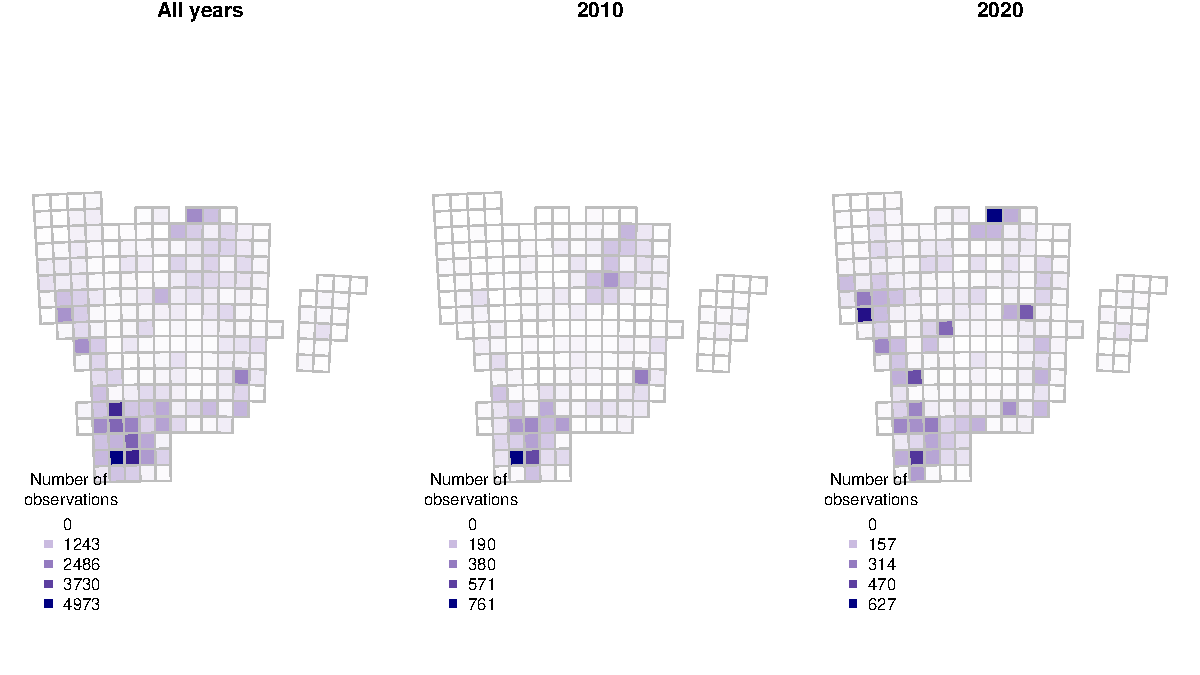
\includegraphics{r-tools-tutorial_files/figure-latex/plotBIRDSspatial-1.pdf}

\begin{Shaded}
\begin{Highlighting}[]
\FunctionTok{suppressWarnings}\NormalTok{(}\FunctionTok{par}\NormalTok{(oldpar))}
\end{Highlighting}
\end{Shaded}

\begin{Shaded}
\begin{Highlighting}[]
\FunctionTok{library}\NormalTok{(sf)}
\end{Highlighting}
\end{Shaded}

\begin{verbatim}
## Warning: package 'sf' was built under R version 4.0.5
\end{verbatim}

\begin{verbatim}
## Linking to GEOS 3.9.0, GDAL 3.2.1, PROJ 7.2.1
\end{verbatim}

\begin{Shaded}
\begin{Highlighting}[]
\FunctionTok{library}\NormalTok{(cowplot)}
\end{Highlighting}
\end{Shaded}

\begin{verbatim}
## Warning: package 'cowplot' was built under R version 4.0.3
\end{verbatim}

\begin{Shaded}
\begin{Highlighting}[]
\FunctionTok{library}\NormalTok{(ggplot2)}
\FunctionTok{library}\NormalTok{(colorRamps)}
\end{Highlighting}
\end{Shaded}

\begin{verbatim}
## Warning: package 'colorRamps' was built under R version 4.0.3
\end{verbatim}

\begin{Shaded}
\begin{Highlighting}[]
\NormalTok{spatial\_sf }\OtherTok{\textless{}{-}} \FunctionTok{st\_as\_sf}\NormalTok{(SB}\SpecialCharTok{$}\NormalTok{spatial)}

\NormalTok{obs }\OtherTok{\textless{}{-}} \FunctionTok{ggplot}\NormalTok{(}\AttributeTok{data =}\NormalTok{ spatial\_sf, }\FunctionTok{aes}\NormalTok{( }\AttributeTok{fill =}\NormalTok{ nVis))}\SpecialCharTok{+}
  \FunctionTok{geom\_sf}\NormalTok{()}\SpecialCharTok{+}
  \FunctionTok{ggtitle}\NormalTok{(}\StringTok{"Visits"}\NormalTok{)}\SpecialCharTok{+}
  \FunctionTok{scale\_fill\_gradient}\NormalTok{(}\AttributeTok{low =} \StringTok{"\#56B1F7"}\NormalTok{,}
                      \AttributeTok{high =} \StringTok{"\#132B43"}\NormalTok{,}
                      \AttributeTok{na.value =} \ConstantTok{NA}\NormalTok{) }\SpecialCharTok{+}
  \FunctionTok{theme\_cowplot}\NormalTok{()}

\NormalTok{obs}
\end{Highlighting}
\end{Shaded}

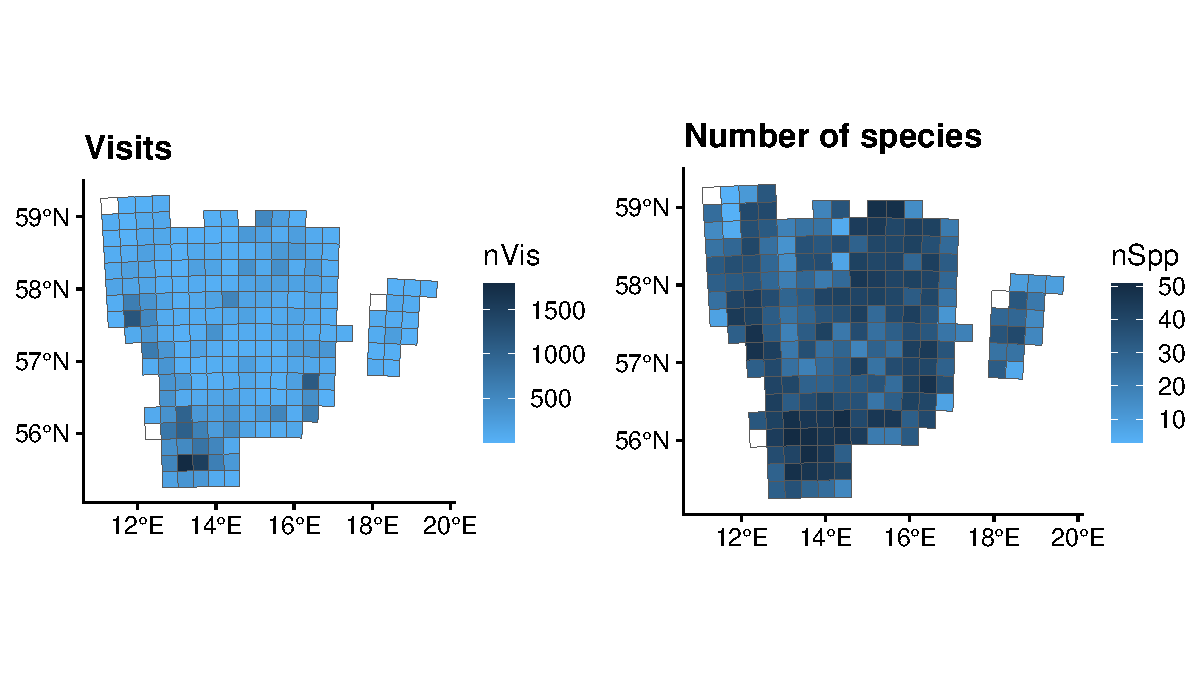
\includegraphics{r-tools-tutorial_files/figure-latex/ggplot1-1.pdf}

\begin{Shaded}
\begin{Highlighting}[]
\NormalTok{spp }\OtherTok{\textless{}{-}} \FunctionTok{ggplot}\NormalTok{(}\AttributeTok{data =}\NormalTok{ spatial\_sf ,}\FunctionTok{aes}\NormalTok{( }\AttributeTok{fill =}\NormalTok{ nSpp))}\SpecialCharTok{+}
  \FunctionTok{geom\_sf}\NormalTok{()}\SpecialCharTok{+}
  \FunctionTok{ggtitle}\NormalTok{(}\StringTok{"Number of species"}\NormalTok{)}\SpecialCharTok{+}
  \FunctionTok{scale\_fill\_gradient}\NormalTok{(}\AttributeTok{low =} \StringTok{"\#56B1F7"}\NormalTok{,}
                      \AttributeTok{high =} \StringTok{"\#132B43"}\NormalTok{,}
                      \AttributeTok{na.value =} \ConstantTok{NA}\NormalTok{) }\SpecialCharTok{+}
  \FunctionTok{theme\_cowplot}\NormalTok{()}

\NormalTok{spp}
\end{Highlighting}
\end{Shaded}

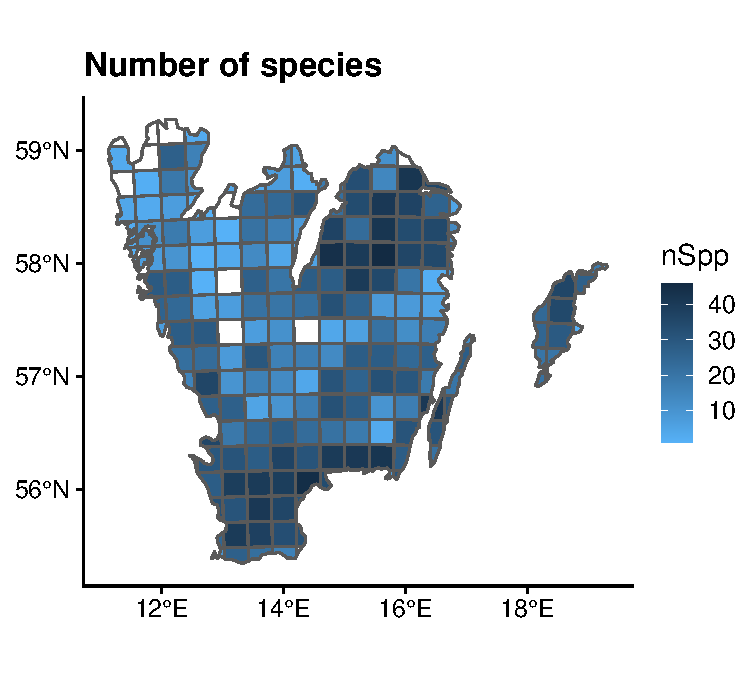
\includegraphics{r-tools-tutorial_files/figure-latex/ggplot2-1.pdf}

How has observation effort (frequency of visits) varied over time and space? -- 1) show maps as in Example 7 (all years, year 2000, 2002, 2004, 2006, 2008, 2010), 2 make also a time line plot with no. visits against years, no. of gridcells with visits against years.

we see that SB contains an element called \texttt{SB\$temporal} that contains a daily time series with time specific rows when there is information. \texttt{xts} also supports time, but dating below day resolution is not yet implemented in the \texttt{BIRDS} package.

\begin{Shaded}
\begin{Highlighting}[]
\NormalTok{sb.xts }\OtherTok{\textless{}{-}}\NormalTok{ SB}\SpecialCharTok{$}\NormalTok{temporal}
\FunctionTok{head}\NormalTok{(sb.xts)}
\end{Highlighting}
\end{Shaded}

\begin{verbatim}
##            nObs nVis nSpp
## 2000-03-24    1    1    1
## 2000-04-05    4    3    3
## 2000-04-06   11    6    3
## 2000-04-10    1    1    1
## 2000-04-12    3    3    1
## 2000-04-13    8    5    2
\end{verbatim}

\begin{Shaded}
\begin{Highlighting}[]
\FunctionTok{dim}\NormalTok{(sb.xts)}
\end{Highlighting}
\end{Shaded}

\begin{verbatim}
## [1] 1118    3
\end{verbatim}

Sub-setting is convenient in \texttt{xts} as you can do it with its dates and with a \texttt{/} for a range of dates.

\begin{Shaded}
\begin{Highlighting}[]
\NormalTok{sb.xts[}\StringTok{"2010{-}09"}\NormalTok{] }\CommentTok{\#a specific month}
\end{Highlighting}
\end{Shaded}

\begin{verbatim}
##            nObs nVis nSpp
## 2010-09-01   38   15   14
## 2010-09-02   26   12   12
## 2010-09-03   20    9   10
## 2010-09-04   63   19   18
## 2010-09-05   71   25   12
## 2010-09-06   16    4    9
## 2010-09-07    9    7    5
## 2010-09-08   13    6    8
## 2010-09-09   32   12   14
## 2010-09-10    1    1    1
## 2010-09-11   15    8    8
## 2010-09-12   15    7    8
## 2010-09-13   14    5    9
## 2010-09-14    1    1    1
## 2010-09-15    3    3    2
## 2010-09-17    3    2    3
## 2010-09-18    9    5    5
## 2010-09-19   12    7    5
## 2010-09-21    3    2    3
## 2010-09-22    4    4    2
## 2010-09-23    3    3    2
## 2010-09-24   10    5    5
## 2010-09-25    6    3    6
## 2010-09-26    7    6    2
## 2010-09-28    2    2    2
## 2010-09-29    5    3    4
## 2010-09-30    2    2    2
\end{verbatim}

\begin{Shaded}
\begin{Highlighting}[]
\NormalTok{sb.xts[}\StringTok{"2010{-}09{-}07"}\NormalTok{] }\CommentTok{\#a specific day}
\end{Highlighting}
\end{Shaded}

\begin{verbatim}
##            nObs nVis nSpp
## 2010-09-07    9    7    5
\end{verbatim}

\begin{Shaded}
\begin{Highlighting}[]
\NormalTok{sb.xts[}\StringTok{"2007{-}01{-}01/2007{-}05{-}01"}\NormalTok{] }\CommentTok{\#for a period}
\end{Highlighting}
\end{Shaded}

\begin{verbatim}
##            nObs nVis nSpp
## 2007-03-05    1    1    1
## 2007-03-14    1    1    1
## 2007-03-20    4    4    4
## 2007-04-02    7    4    4
## 2007-04-11   14    7    3
## 2007-04-12    8    6    4
## 2007-04-13    1    1    1
## 2007-04-15    1    1    1
## 2007-04-17    6    4    3
## 2007-04-18    1    1    1
## 2007-04-21    1    1    1
## 2007-04-23    1    1    1
## 2007-04-27   11    6    4
## 2007-04-28    4    4    3
## 2007-04-30    2    2    2
\end{verbatim}

The package \texttt{xts} has several tools for converting to different periods. Here we will use \texttt{to.monthly}. This provides, the first, min, max, and last of the data. We can plot the daily maximum number of observations. The plot command with an \texttt{xts} object provides a TON of features. This makes it fairly easy to customize your plots. Read more in \texttt{?plot.xts}.

\begin{Shaded}
\begin{Highlighting}[]
\FunctionTok{library}\NormalTok{(xts)}
\NormalTok{obs.m }\OtherTok{\textless{}{-}} \FunctionTok{to.monthly}\NormalTok{(sb.xts}\SpecialCharTok{$}\NormalTok{nObs) }
\NormalTok{obs.m[}\StringTok{"2007{-}04"}\NormalTok{]}
\end{Highlighting}
\end{Shaded}

\begin{verbatim}
##          sb.xts$nObs.Open sb.xts$nObs.High sb.xts$nObs.Low sb.xts$nObs.Close
## Apr 2007                7               14               1                 2
\end{verbatim}

\begin{Shaded}
\begin{Highlighting}[]
\NormalTok{sb.xts[}\StringTok{"2007{-}04"}\NormalTok{]}
\end{Highlighting}
\end{Shaded}

\begin{verbatim}
##            nObs nVis nSpp
## 2007-04-02    7    4    4
## 2007-04-11   14    7    3
## 2007-04-12    8    6    4
## 2007-04-13    1    1    1
## 2007-04-15    1    1    1
## 2007-04-17    6    4    3
## 2007-04-18    1    1    1
## 2007-04-21    1    1    1
## 2007-04-23    1    1    1
## 2007-04-27   11    6    4
## 2007-04-28    4    4    3
## 2007-04-30    2    2    2
\end{verbatim}

\begin{Shaded}
\begin{Highlighting}[]
\FunctionTok{plot}\NormalTok{(obs.m[}\StringTok{"2000/2010"}\NormalTok{,}\DecValTok{2}\NormalTok{], }\AttributeTok{col =} \StringTok{"darkblue"}\NormalTok{, }\AttributeTok{grid.ticks.on =} \StringTok{"month"}\NormalTok{, }
     \AttributeTok{major.ticks =} \StringTok{"month"}\NormalTok{, }\AttributeTok{grid.col =} \StringTok{"lightgrey"}\NormalTok{,  }
     \AttributeTok{main =} \StringTok{"Maximum number of daily observations per month"}\NormalTok{)}
\end{Highlighting}
\end{Shaded}

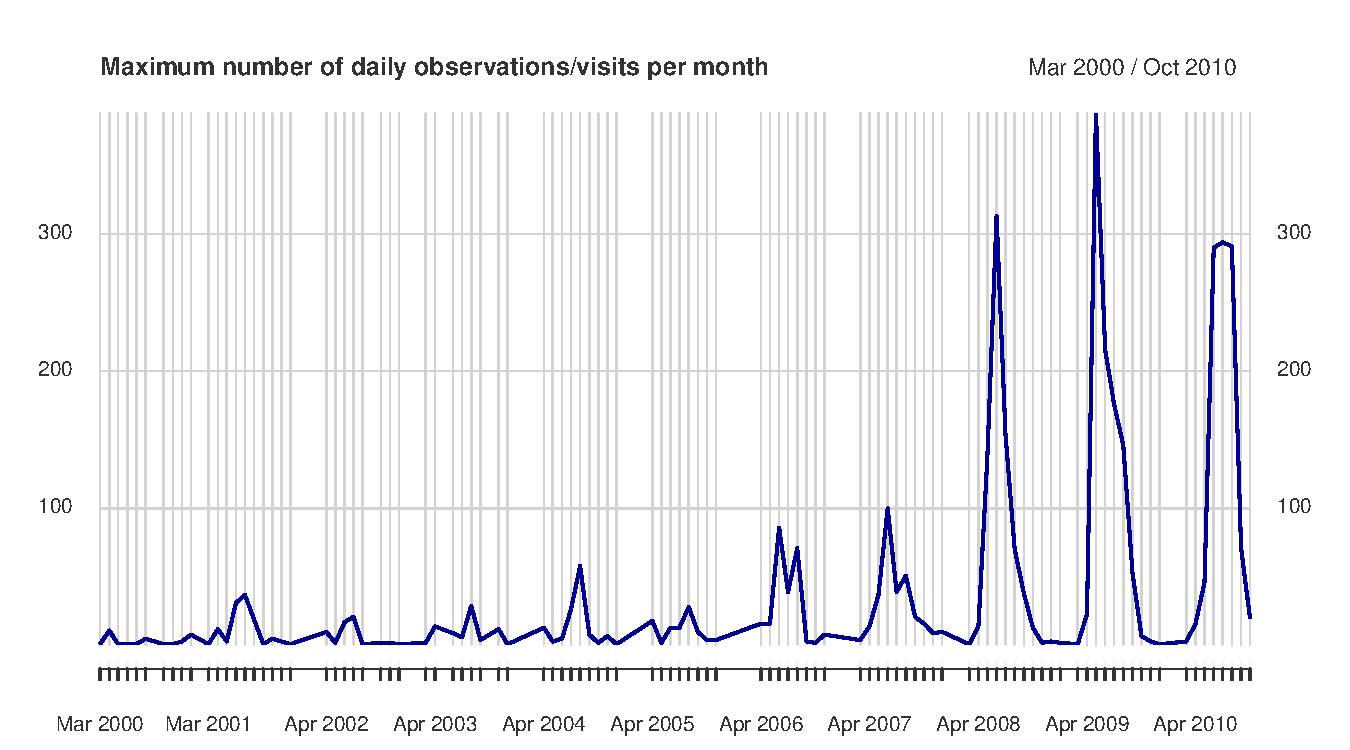
\includegraphics{r-tools-tutorial_files/figure-latex/monthly and plot-1.pdf}

\begin{Shaded}
\begin{Highlighting}[]
\NormalTok{vis.m }\OtherTok{\textless{}{-}} \FunctionTok{to.monthly}\NormalTok{(sb.xts}\SpecialCharTok{$}\NormalTok{nVis) }
\NormalTok{vis.m[}\StringTok{"2007{-}04"}\NormalTok{]}
\end{Highlighting}
\end{Shaded}

\begin{verbatim}
##          sb.xts$nVis.Open sb.xts$nVis.High sb.xts$nVis.Low sb.xts$nVis.Close
## Apr 2007                4                7               1                 2
\end{verbatim}

\begin{Shaded}
\begin{Highlighting}[]
\NormalTok{sb.xts[}\StringTok{"2007{-}04"}\NormalTok{]}
\end{Highlighting}
\end{Shaded}

\begin{verbatim}
##            nObs nVis nSpp
## 2007-04-02    7    4    4
## 2007-04-11   14    7    3
## 2007-04-12    8    6    4
## 2007-04-13    1    1    1
## 2007-04-15    1    1    1
## 2007-04-17    6    4    3
## 2007-04-18    1    1    1
## 2007-04-21    1    1    1
## 2007-04-23    1    1    1
## 2007-04-27   11    6    4
## 2007-04-28    4    4    3
## 2007-04-30    2    2    2
\end{verbatim}

\begin{Shaded}
\begin{Highlighting}[]
\FunctionTok{plot}\NormalTok{(vis.m[}\StringTok{"2000/2010"}\NormalTok{,}\DecValTok{2}\NormalTok{], }\AttributeTok{col =} \StringTok{"darkblue"}\NormalTok{, }\AttributeTok{grid.ticks.on =} \StringTok{"month"}\NormalTok{, }
     \AttributeTok{major.ticks =} \StringTok{"month"}\NormalTok{, }\AttributeTok{grid.col =} \StringTok{"lightgrey"}\NormalTok{, }
     \AttributeTok{main =} \StringTok{"Maximum number of daily visits per month"}\NormalTok{)}
\end{Highlighting}
\end{Shaded}

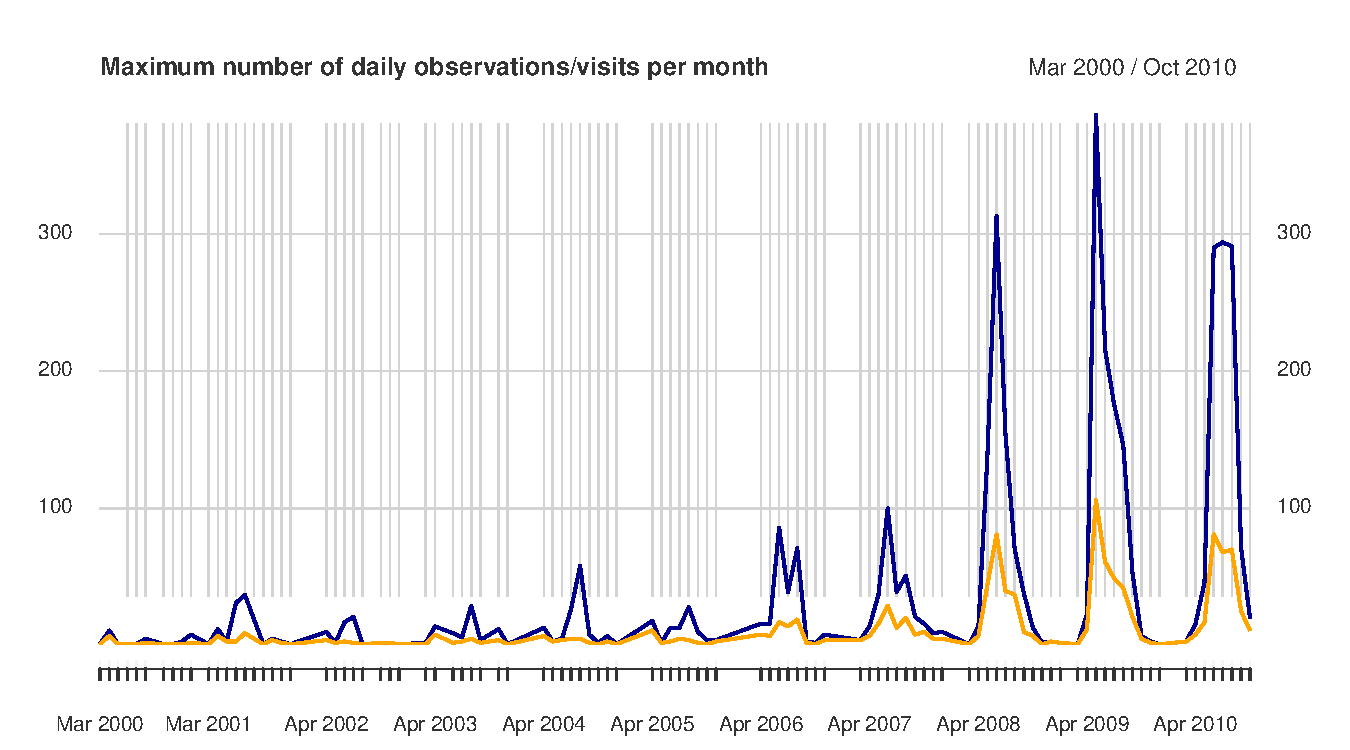
\includegraphics{r-tools-tutorial_files/figure-latex/monthly and plot-2.pdf}

We can now look at some particular species and ask whether this has changed in occurrence over time:
Plot no. records of species x and no. visits all species over years (we simply explore by comparing records for a species with no visits, can assume that species has increased of stronger positive trend than for no. visits)

Plot no. gridcells with visits for species x and no. gridcells with visits for all species over years (we simply explore by comparing records for a species with no visits, can assume that species has increased of stronger positive trend than for no. visits)
(species x: Tvåfläckad trollslända Epitheca bimaculata)

  \bibliography{references.bib}

\end{document}
